\documentclass[a4paper, 12pt, ngerman, twoside, openright]{scrreprt}

% Rendering packages
\usepackage{amsmath}
\usepackage{amssymb}
\usepackage{graphicx, float}
\usepackage{color}
\usepackage{fancyvrb}
\usepackage{pdfpages}

% Page dimensions
\usepackage[inner=3.5cm,outer=2.5cm,top=3.7cm,bottom=3.5cm]{geometry} % Settings for twoside documents.
\usepackage{parskip}

% Font styling
\usepackage[ngerman]{babel}
\usepackage[utf8]{inputenc}
\usepackage[T1]{fontenc}
\usepackage{lmodern}
\renewcommand\familydefault{\sfdefault}

% Tables
\usepackage{tabularx}
\usepackage{tabulary}
\usepackage{longtable, lscape}

% Headers
\usepackage{scrpage2}  % header and footer for KOMA-Script
\pagestyle{scrheadings}
\automark[section]{chapter}
\usepackage{marvosym} % für Euro-Zeichen

% Zitate
\usepackage[backend=bibtex, style=numeric, sorting=none]{biblatex}
\usepackage[babel,german=guillemets]{csquotes}
\bibliography{Bibliothek/Bibliothek}

\usepackage[hyperindex,breaklinks,colorlinks=true,linkcolor=black,urlcolor=blue,citecolor=black]{hyperref}

% Code Blöcke
\usepackage{listings}

% Listings konfigurieren.
\lstset{language=[Objective]C, 
        breakindent=40pt, 
        breaklines, 
        frame=lines,
        morekeywords={id, Class, SEL, IMP, BOOL, nil, Nil, NO, YES,
                  oneway, in, out, inout, bycopy, byref,
                  self, super, _cmd,
                  @required, @optional,
                  @try, @throw, @catch, @finally,
                  @synchronized, @property, @synthesize, @dynamic},
        basicstyle=\ttfamily\scriptsize,
        literate=
            {Ö}{{\"O}}1
            {Ä}{{\"A}}1
            {Ü}{{\"U}}1
            {ß}{{\ss}}2
            {ü}{{\"u}}1
            {ä}{{\"a}}1
            {ö}{{\"o}}1}
        
\definecolor{dkgreen}{rgb}{0,0.6,0}
\definecolor{gray}{rgb}{0.5,0.5,0.5}
\definecolor{mauve}{rgb}{0.58,0,0.82}
\definecolor{orange}{rgb}{1,0.35,0.2}
\definecolor{lightblue}{rgb}{0.53,0.81,0.98}        

\lstset{frame=tb,
	language=Java,
	aboveskip=3mm,
	belowskip=3mm,
	showstringspaces=false,
	columns=flexible,
	basicstyle={\small\ttfamily},
	numbers=none,
	numberstyle=\tiny\color{gray},
	keywordstyle=\color{blue},
	commentstyle=\color{dkgreen},
	stringstyle=\color{mauve},
	breaklines=true,
	breakatwhitespace=true,
	tabsize=3
}

\lstdefinelanguage{drools}{frame=tb,
	morekeywords={rule, rule, when,then, end, end}
	aboveskip=3mm,
	belowskip=3mm,
	showstringspaces=false,
	columns=flexible,
	basicstyle={\small\ttfamily},
	numbers=none,
	numberstyle=\tiny\color{lightblue},
	keywordstyle=\color{orange},
	breaklines=true,
	breakatwhitespace=true,
	tabsize=4}

%NEW COMMANDS
\newcommand\tab[1][1cm]{\hspace*{#1}}

%Verfickte Glossare
\usepackage[nonumberlist,acronym,toc]{glossaries}
\makeglossaries
\newacronym[]{BSP}{BSP}{Beispiel Abkürzung}

\newglossaryentry{Beispiel Glossary Entry}
{
  name=Constrain-Satisfaction-Problem,
  description={Ein Constraint-Satisfaction-Problem besteht aus einer Menge von Variablen, ihren Wertebereichen und den Bedingungen, die Verknüpfungen zwischen den Variablen herstellen und dadurch festlegen, welche Kombinationen von Werten der Variablen zulässig sind}
}



\begin{document}



% Titelseite manuell einfügen.

% Counter zurücksetzen. Römische Ziffern einstellen.
%\pagenumbering{Roman}
%\setcounter{page}{1}

% Selbständigkeitserklärung manuell einfügen.

% Abstract einfügen.
\chapter*{Abstract}

Die vorliegende Masterarbeit analysiert den aktuellen Stand der Digitalisierung im Handwerk, sowie kleinen und mittleren Unternehmen und findet auf dieser Grundlage Bereiche, die Unterstützung benötigen. Darauf basierend wird ein Augmented Reality Applikation für Fliesenleger entwickelt und ihr Mehrwert für Handwerker bestimmt. Durch eine Fokusgruppe und eine Ethnographie werden Daten zu Problemen von Handwerkern erhoben und Ansätze für ein Unterstützungswerkzeug gefunden. Daraus wird eine Microsoft HoloLens Applikation für Fliesenleger mithilfe von gestaltungsorientierter Forschung implementiert, welche anschließend mit Handwerkern durch einen Fragebogen und ein Interview evaluiert wird. Die Ergebnisse bestätigen die Annahme, dass Augmented Reality als Visualisierungswerkzeug für Kundengespräche und zur Unterstützung bei der Arbeit für Handwerker interessant ist. Schlussfolgernd lässt sich sagen, dass Datenbrillen für Augmented Reality noch nicht genügend ausgereift sind, in Zukunft jedoch für Handwerker interessant sein können.

The present master thesis analyses the current state of digitisation in crafts, as well as small and medium-sized enterprises, and on this basis finds areas that require support. Based on this, an Augmented Reality application for tilers will be developed and its added value for craftsmen will be determined. Through a focus group and an ethnography data on problems of craftsmen will be collected and approaches for a support tool will be found. From this, a Microsoft HoloLens application for tilers will be implemented using design science, which will then be evaluated with craftsmen through a questionnaire and an interview. The results confirm the assumption that Augmented Reality is interesting for craftsmen as a visualization tool, for advising customers and to support their work. In conclusion, it can be said that head mounted displays for augmented reality are not yet sufficiently mature, but may be interesting for craftsmen in the future.

% Inhaltsverzeichnis generieren.
\tableofcontents

% Neue Seite. Counter zurücksetzen. Arabische Ziffern einstellen.
\cleardoublepage
\pagenumbering{arabic}
\setcounter{page}{1}

% Kapitel einfügen.
\chapter{Einleitung}

In unserem modernen Zeitalter schreitet die Technik immer weiter voran. In den letzten zwei Jahrzehnten ist im Bereich Computer und Technologie so viel erreicht worden, wie niemand für möglich gehalten hatte. Jedes Jahr treten wieder neue Technologien und Gadgets in das Leben der Menschen und die Einsatzmöglichkeiten und das Potenzial scheinen schier unendlich. Diese Neuerungen finden nicht nur im privaten Gebrauch großen Anklang, sondern bieten besonders Unternehmen viele Möglichkeiten sich weiterzuentwickeln, neue Produkte herzustellen und Kosten zu sparen. Wie in der Industrialisierung die Dampfmaschine, verhelfen heute technische Geräte und Computerchips den Unternehmen dabei, Arbeiten effizienter zu bewerkstelligen. Sie ermöglichen das Einbinden, sowie die Kontrolle und Optimierung neuer Prozesse. Teilweise fühlt es sich sogar an, als wären diese Computer bald schlauer als der Mensch und ersetzen ihn so bei der Arbeit. Im Vordergrund jedoch steht, dass diese Geräte die Arbeit unterstützen und so zum Wirtschaftswachstum beitragen. \\
Große Unternehmen nutzen diese Neuerungen mehr zu ihrem Vorteil, als kleine oder mittlere Unternehmen (\textbf{KMU}) oder Handwerksbetriebe \cite{hateful_six_krcmar}. Durch ihre Flexibilität und weniger Bürokratie ist das Potential für Digitalisierung gegeben, allerdings wird dieses aufgrund der Risiken oft nicht genutzt. Handwerksbetriebe beispielsweise nutzen kaum technische Assistenzsystem und  setzen noch immer auf papierbasierte Anleitungen anstatt z.B. mit Tablets zu arbeiten \cite{zheng_eye-wearable_2015}. Diese wären aber für den Einsatz auf einer rauen Baustelle nicht geeignet. Für die Produktionsunterstützung oder in Werkstätten werden sie jedoch häufig genutzt. \\
Neue Entwicklungen in der Augmented Reality (\textbf{AR}) mit Apparaten, die direkt am Körper getragen werden können \cite{zheng_eye-wearable_2015} sehen dafür vielversprechend aus. Datenbrillen, wie Google Glass oder die Microsoft HoloLens haben insofern hohes Potential, da Nutzer bei der Verwendung die Hände frei haben. Diese AR Brillen projizieren Hologramme in die reale Umgebung des Nutzers und lassen so Realität und virtuelle Welt verschmelzen. Dadurch können Nutzern Informationen eingeblendet werden, mit welchen sie per Gesten- oder Sprachsteuerung interagieren können. Da sie die Geräte auf dem Kopf tragen, bleiben ihre Hände frei um Aktionen, wie Reparaturen auszuführen. Besonders die Microsoft HoloLens überzeugt hier mit ihrem großen Speicher, was es ermöglicht komplexe Programme aufzuspielen und diese auch Offline und unterwegs zu nutzen.

Die Ziele dieser Arbeit sind es, den \textit{momentanen Stand der Digitalisierung in KMUs und Handwerksbetrieben zu bestimmen}, eine \textit{Augmented Reality Applikation für Handwerker zu designen und zu implementieren} und den \textit{Mehrwert von AR Applikationen für das Handwerk zu bestimmen}. \\
Anfangs wird erforscht, warum KMUs und Handwerksbetriebe wenig digitalisieren, ob AR von ihnen bereits verwendet wird oder sie darin überhaupt Potenzial sehen. Daraus soll hervorgehen, wo der Einsatz von AR gefragt ist. \\

\chapter{Hintergrund}

Dieses Kapitel legt den Grundstein für diese Arbeit. Es liefert den theoretischen Hintergrund, sowie die Motivation für die Forschung zur Digitalisierung im Handwerk. Zuerst wird der Stand der Digitalisierung in Handwerksbetrieben, sowie kleinen und mittleren Unternehmen dargelegt, welcher Anreiz gegeben hat, dieses Thema genauer zu beleuchten. Anschließend wird herausgearbeitet, wie digitale Anwendungen bereits eingesetzt werden, um bei bestimmten Arbeitsschritten zu unterstützen. Dabei werden Spezifikationserstellung und Dienstleistungsunterstützung genauer betrachtet und mit Beispielen veranschaulicht. Zuletzt wird auf das Potenzial von Augmented Reality zur Visualisierung eingegangen und dies wiederum durch Beispielanwendungen veranschaulicht.

\section{Digitalisierung in Handwerksbetrieben, kleinen und mittleren Unternehmen}

Die Digitalisierung hält Einzug in den meisten Branchen, was in dieser modernen Zeit, in welcher auch im privaten Leben mehr und mehr Technik zum Einsatz kommt, nicht verwunderlich ist. Mithilfe neuer Technologien und Programmen lassen sich beispielsweise Abläufe beschleunigen, Genauigkeit und Effizienz verbessern, sowie die Erreichbarkeit steigern. Oft werden diese Technologien zum bewältigen des Verwaltungsaufwands genutzt, was kleinen und mittleren Unternehmen (\textbf{KMUs}), als auch Handwerksbetrieben mehr Zeit für ihre eigentliche Aufgabe lässt: das Handwerk \cite{noauthor_neue_nodate}. Unternehmen wollen sich diese neuen Chancen zu nutze machen und Investieren dazu in Umrüstung und Umstrukturierung von Unternehmensabläufen, sowie in die Integration von neuen Programmen und technischen Hilfsmitteln in ihr Arbeitsumfeld \cite{TODO: Buchkapitel}. Große, kommerzielle Unternehmen fällt das leichter als KMUs und Handwerksbetrieben \cite{hateful_six_krcmar}.

KMUs spielen aber ein wichtige Rolle in unserer Gesellschaft und Wirtschaft, weshalb ihr langsamer Fortschritt im Bereich Digitalisierung auf keinen Fall leicht zu nehmen ist. In den USA beispielsweise stellen KMUs 95\% aller Unternehmen und sind verantwortlich für zwei Drittel aller neuen Arbeitsplätze. Zusätzlich werden 60\% des Exports von ihnen gestemmt \cite{allocca_innovation_2006}. Diese Argumente machen KMUs zu einem lohnenswerten und interessanten Forschungsgebiet, was sich in den letzten Jahren auch deutlich zeigte.

Fries et al. \cite{hateful_six_krcmar} trug durch ihre Forschung sechs Faktoren zusammen, welche dafür verantwortlich sind, dass KMUs ihren größeren Konkurrenten in der Digitalisierung hinterher hängen. Das liegt an: 

\begin{enumerate}
	\item einem empfundenen Ungleichgewicht zwischen Risiken und Möglichkeiten,
	\item mangelnder Vereinbarkeit mit der täglichen Arbeitsroutine,
	\item einer schwierigen Eingliederung in individuelle Geschäftsprozesse,
	\item komplexen Infrastrukturinvestitionen,
	\item nicht oder kaum vorhandenem IT Knowhow und
	\item hohen Installationskosten für die Inbetriebnahme der neuen Technologien.
\end{enumerate}

KMUs denken bei dem Einsatz von neuen Technologien vermehrt an Risiken und Kosten, als an Chancen, die daraus entstehen oder andere positive Aspekte. Sie haben limitierte Ressourcen an Kapital und Arbeitskräften und können sich daher keine falschen Entscheidungen oder Investitionen erlauben \cite{allocca_innovation_2006}. Mit dem Adaptieren und Einsatz von Innovationen geht immer ein hohes finanzielles Risiko einher. KMUs können, im Gegensatz zu größeren Firmen, diese Kosten meist nicht über mehrere Projekte verteilen, um die Belastung zu minimieren \cite{rothwell_small_1989}. \\
Alloca und Kessler \cite{allocca_innovation_2006} wiederum schreiben KMUs mehr Risikobereitschaft zu, da das Management bzw. die Geschäftsführung meist aus Entrepreneurs besteht, die den Einstieg in die Industrie durch Wagnisse schaffen wollen oder geschafft haben. Ein solches Unternehmen muss, aufgrund der knapperen Ressourcen, schneller und effizienter arbeiten, um konkurrenzfähig zu bleiben.

Des weiteren spielt es eine große Rolle, ob neue Technologien den Arbeitsalltag tatsächlich erleichtern und wie diese von den Mitarbeitern aufgenommen und in ihre Routine integriert werden. Dies kann besonders bei älteren Mitarbeitern, die \textit{"schon immer so gemacht"} haben schwierig werden. Die Arbeitsprozesse müssen umgebaut werden, um die neuen Geräte oder Programme zu unterstützen und ihre Potential zu nutzen. Da oft niemand vorhanden ist, der sich ausschließlich mit \textit{Research \& Development} beschäftigt, sind diese Entscheidungen schwer zu treffen \cite{rothwell_small_1989}. Nichtsdestotrotz haben KMUs aufgrund weniger Bürokratie das Potenzial, schneller Änderungen zu adaptieren (\cite{kessler_innovation_1996} und \cite{kessler_speeding_1999}, zitiert in \cite{allocca_innovation_2006}).

Unternehmerische Manager können oft die steigende Komplexität der Firma, durch deren Wachstum und Integration von neuen Technologien, schwer überblicken, worunter die Eingliederungen von Neuerungen in Geschäftsprozesse leidet \cite{rothwell_small_1989}. Dafür sind weniger standardisierte Prozesse und Guidlines, ein weniger systematischer Management Style und generell die geringere Erfahrung des Managements im Vergleich zu großen Unternehmen verantwortlich \cite{allocca_innovation_2006}. 

Das Einbinden der neuen Technologien in die bestehende Infrastruktur des Unternehmens stellt zusätzliche Risiken und Kosten dar. Der Arbeitsplatz war meist ursprünglich nicht dafür designed, um schnell und einfach neue Geräte oder Programme zu integrieren. Teilweise lässt auch der Ort an dem gearbeitet wird den Einsatz generell nicht oder nur bedingt zu. Auf einer Baustelle oder in einem Kellergewölbe beispielsweise kann keine permanente WLAN Verbindung sichergestellt werden \cite{TODO: Buchkapitel}. Dadurch wird der Einsatz von digitalen Medien erschwert.

Da KMUs und vor allem Handwerksbetriebe oft aus wenigen Mitarbeitern bestehen, ist die Wahrscheinlichkeit hoch, dass kein Technikspezialist an Board ist. Das macht es nötig, sich fremde Expertise einzuholen, um in die richtige Technologie für den Betrieb zu investieren. Jedoch bringt das zusätzliche Kosten und Zeitaufwand mit sich, welche oft nicht verfügbar sind \cite{rothwell_small_1989}. Des weiteren müssen die Mitarbeiter für die neue Technologie geschult werden, wodurch wieder Zeit verloren geht. Fehler, die durch Anschaffung falscher technischer Hilfsmittel, oder durch unsachgemäßen, ineffizienten Einsatz dieser entstehen, kosten unnötig Geld. Das kann sich ein Unternehmen mit begrenzten Ressourcen nicht leisten \cite{allocca_innovation_2006}.

Die Schulung der Mitarbeiter ist durchaus zeit- und kostenaufwändig. Aber auch die Anschaffung und Installation der neuen Technologie birgt eine finanzielle Hürde für die Unternehmen. Zusätzliche, versteckte Kosten welche durch Probleme mit Patenten oder Auflagen des Staates entstehen, stellen eine große Belastung bei der Integration dar \cite{rothwell_small_1989}. 

Trotz dieser Hindernden Faktoren für KMUs und Handwerksbetriebe bieten sich viele Möglichkeiten für diese. Ritchie und Brindley \cite{ritchie_ict_2005} sehen großes Potential für diese Unternehmen im Bereich Digitalisierung mit ihren kommerziellen Konkurrenten mitzuhalten, da sie \textit{flexibler, effizienter und adaptiver} sind, was Grundvoraussetzungen für die Integration von Neuerungen ist. \\
Das bereits Produkte zur Unterstützung für Handwerksbetriebe und KMUs existieren und genutzt werden, wird im Folgenden genauer dargestellt.

\section{Unterstützung der Spezifikationserstellung mit digitalen Anwendungen}
\label{sec:spezi}

''Auf Baustellen müssen sich Kunde und Handwerker erst einig werden, was genau getan werden soll, denn ''[g]erade im Dienstleistungsbereich gibt es einen engen Zusammenhang zwischen hoher Kundenzufriedenheit und dem Einbinden des Kunden''.'' (\cite{TODO: Buchkapitel}, zitiert nach \cite{hentrich_arbeiten_2002}). Die Kommunikation des Plans gestaltet sich dabei oft schwierig. Ein Problem, das viele Handwerker anmerken (siehe Fokusgruppe \ref{sec:fokus}) ist, dass Kunden wenig Vorstellungsvermögen haben. Der Handwerker, als Experte, kann einen Raum betreten und sich direkt vorstellen, wie er diesen gestalten würde. Dies dem Kunden nur durch Worte zu kommunizieren ist jedoch schwierig. Dadurch kann der Handwerker den Kunden nicht effektiv beraten und dieser kann wiederum schwer seine Vorstellungen beschreiben. Verschiedene Werkzeuge können dabei helfen, dies zu veranschaulichen.

Traditionell werden Baupläne und Blaupausen auf Papier in 2D gezeichnet \cite{TODO: Buchkapitel}. Der technische Zeichner kann so ganze Gebäude bis ins kleinste Detail spezifizieren und sogar mit Inneneinrichtung ausstatten. Diese Methode hat jedoch zum Nachteil, dass zum Lesen der Pläne sehr viel Erfahrung erforderlich ist. Gleichzeitig sind diese, aufgrund ihrer Komplexität, auch für erfahrene Handwerker fehleranfällig und führen zu Fehlern bei der Umsetzung \cite{wang_using_2007}. Für den Kunden bringt die Verwendung dieser Pläne kaum einen Vorteil bezüglich des Verständnisses. Die Zeichnungen sind technisch komplex, können von Laien nur mäßig verstanden werden und tragen dadurch nur mäßig zu einer besseren Kunde-Handwerker-Kommunikation bei.

Es wird also ein Mittel oder Werkzeug benötigt, dass diese Verständigung und somit auch die Spezifikation und den Vertragsschluss unterstützt. Es soll dabei den Kunden unterstützen die Pläne des Handwerkers besser zu verstehen und sich vorstellen zu können. Dafür muss es geeignete Visualisierungsmethoden mitbringen, um den Plan verständlich darzustellen. \\
Der Kunde kann anhand des ihm gezeigten Bildes besser Änderungen Vorschlagen. So kann er deutlicher Änderungsvorschläge bringen, zeigen wo er sie Anbringen möchte und erleichtert damit das Kundengespräch für beide Parteien. \\
Es ermöglicht auch dem Handwerker einfach verständlicher Ratschläge zu geben und gezielt auf Details einzugehen. Dies steigert zusätzlich die vom Kunden empfundene Kompetenz des Handwerkers, da er direkt sehen kann, was die Pläne des Handwerkers sind und sich besten Fall vorstellen kann, wie das Endergebnis aussieht. \\
Anschließend werden einige, teils kommerzielle, Spezifikationswerkzeuge vorgestellt, die diesen Zielen genügen.

\begin{figure}[H]
	\begin{center}
		\includegraphics[scale=0.65]{Resources/Hintergrund/sketchup.jpg}
		\caption{3D Modellierter Bauplan in SketchUp 3D}
	\end{center}
\end{figure}

SketchUp 3D ist eine 3D-Modellierungssoftware, die 2D hand- oder computergezeichnete Baupläne zugänglicher machen kann. Dazu ermöglicht es die teilweise Umwandlung dieser 2D Zeichnungen in 3D Modelle. Bilder werden in SketchUp eingefügt, mit zusätzlichen Informationen versehen und erweitert. Eine der Funktionalitäten ist es beispielsweise eine Wand zu markieren und diese ''aus der Zeichnung heraus zu ziehen''. So erstellt das Programm ein 3D Modell des Raums, durch das sie der Kunde am Computer bewegen kann. Gleiches kann auf Tische und Ähnliches angewandt werden. Zusätzlich ist es möglich, Texturen auf Objekte zu legen. Der Nutzer kann damit den Wänden die Farbe geben, die der echte Raum hat, oder mit verschiedenen Designs experimentieren, um seine gewünschte Stimmung zu erhalten. Dadurch bekommt der Kunde ein Gefühl dafür, wie das Endergebnis aussehen kann. \\
Robert M. Wolk \cite{wolk_utilizing_2008} nutzt SketchUp 3D in Kombination mit Google Earth, um Bürgern mehr Mitbestimmungsrecht bei der Planung eines Windparks zu geben. Dafür erstellt er den Windpark in SketchUp und fügt diesen in Google Earth an der geplanten Bauposition ein (siehe Abbildung \ref{windfarm}). Die Bürger können diesen nun über Google Earth aus ihrer eigenen Perspektive betrachten und abwägen, welche Auswirkungen dieser auf ihr zu Hause oder ihren Arbeitsplatz haben wird. Dadurch können sie eine besser fundierte Entscheidung treffen, ob sie dafür oder dagegen sind.

\begin{figure}[h]
	\begin{center}
		\noindent\includegraphics[scale=0.6]{Resources/Hintergrund/Windfarm.jpg}
		\label{windfarm}
		\caption{Windfarm Modell in Google Earth}	
	\end{center}
\end{figure}

\begin{figure}[h]
	\begin{center}
		\noindent\includegraphics[scale=0.2]{Resources/Hintergrund/irisVR.jpg}
		\label{irisVR}
		\caption{Kollaboration in irisVR an 3D Modell}	
	\end{center}
\end{figure}

Mit irisVR können Designer ihre, am PC erstellten, Blaupausen und 3D Modelle in Virtual Reality (VR) betrachten. Kunden oder Designer können sich dann, mit Hilfe einer VR-Brille, frei in diesem Raum bewegen. Dadurch, dass er das Objekt von allen Seiten betrachten kann bekommt der Kunde eine gute Vorstellung davon. Außerdem kann der Kunde mit dem Modell in VR interagieren. Mehrere Personen können gleichzeitig per VR auf das Modell zugreifen, es bearbeiten und so über Änderungen kommunizieren (siehe Abbildung \ref{irisVR}). Teilweise ist es möglich 3D Modelle in AR mit Hilfe von Tablets oder Smartphones zu betrachten. Ein Raum, in welchem Objekte abgebildet werden sollen, muss davor genau abgemessen und im Modelling Programm angelegt werden. Objekte die jetzt darin positioniert werden, erscheinen als Hologramme am Tablet in den entsprechenden Positionen. 3D Modelle können aus verschiedenen Design Softwarelösungen eingelesen werden. Momentan unterstützt irisVR beispielsweise Revit, SketchUp, OBJ, Grasshopper oder Rhino \cite{helander_joel_2017}. 

Ein weiteres Werkzeug, welches sehr Kundenbezogen ist, ist der Küchenplaner von Biller. Dieser unterstützt am besten, wenn der Grundriss des Raumes, in welchem eine Küche eingebaut werden soll, bekannt ist, der Kunde jedoch noch keine Vorstellung hat, wie seine Küche aussehen bzw. kosten soll. Er kann die Maße und Wandfarben \enquote{genau wie daheim} setzen und den Raum mit Elementen bestücken. Der Küchenplaner errechnet selbst passende Küchenkombinationen als Vorschläge für diesen Raum, sodass nicht alles von Hand positioniert werden muss. Diese Vorschläge können betrachtet und den Wünschen entsprechend angepasst werden. Gleichzeitig zeigt der Planer Preise an und es können Vorschläge aus verschiedenen Preissegmenten gewählt werden.

\begin{figure}[H]
	\begin{center}
		\noindent\includegraphics[scale=0.5]{Resources/Hintergrund/biller.png}
		\caption{Biller Küchenplaner mit Anpassungsmöglichkeiten}	
	\end{center}
\end{figure}

\begin{figure}[h]
	\begin{center}
		\noindent\includegraphics[scale=0.4]{Resources/Hintergrund/schedule4D.png}
		\caption{Schedule Simulator: Modell und Zeitplan}	
	\end{center}
\end{figure}

Die allseits bekannten und weit verbreiteten CAD Systeme dürfen in dieser Aufzählung natürlich nicht fehlen. Mit Schedule Simulator, einem 4D CAD System, hat Bentley Systems das klassische CAD um eine weitere Dimension erweitert. Damit ist es möglich eine gesamte Baustelle, mit Hauptaugenmerk auf zeitlicher Strukturierung, planen. Der Bauleiter legt damit fest, welche Arbeitsschritte nacheinander ausgeführt werden müssen und Schedule Simulator zeigt ihm dazu ein visuelles Modell der einzelnen Bauphasen. Dafür können 3D Modelle aus verschiedenen CAD Programmen geladen werden. An diese werden Zeitplanungsdaten angehängt und das Programm erstellt daraus eine 4D Simulation der Baustelle und der einzelnen Arbeitsschritte \cite{heesom_trends_2004}. Dadurch hat der Bauleiter den gesamten Zeitplan im Blick und kann schnell Änderungen vornehmen, falls sich etwas verzögert. Gleichzeitig kann er dem Kunden den aktuellen Fortschritt zeigen und weitere Schritte erklären. Das unterstützt bereits bei der Vertragsschließung, da alle Vorgänge genau spezifiziert werden können.

\begin{figure}[h]
	\begin{center}
		\noindent\includegraphics[scale=0.4]{Resources/Hintergrund/paletteSlider.png}
		\label{fotoreal}
		\caption{PaletteCAD: Planungsansicht und Fotorealistik Optik}	
	\end{center}
\end{figure}

Ein weiteres Werkzeug aus dieser Gruppe ist das Inneneinrichtungstool PaletteCAD. Damit lassen sich ganze Zimmer planen, wie beispielsweise ein Bad mit Dusche, Badewanne, etc.. Hauptsächlich wird es von Fliesenlegern und Schreinern verwendet. Das Programm liefert eine riesige Auswahl an Material, wie z.B. Fliesen, welches direkt aus den Datenbanken der Hersteller bezogen und regelmäßig geupdated wird. Die designten Räume können anschließend in Fotorealistik Optik gerendert werden (siehe Abbildung \ref{fotoreal}). Zusätzlich lassen sich Modelle für Schreiner direkt auf eine CNC Maschine übertragen. Die Macher versprechen durch benutzerfreundliches Design eine drastische Zeitersparnis bei der Planung.

\section{Augmented Reality als Visualisierungswerkzeug}

In der Allgemeinheit ist VR schon länger bekannt und verbreitet. Dabei wird der Nutzer aus der Realität in eine virtuelle Welt versetzt und nimmt seine physikalische Umgebung nicht mehr war. Momentan wird diese Technologie hauptsächlich für Computerspiele und Filme genutzt, was sie kommerziell, für private Anwender interessant macht. Zur Unterstützung bei der Arbeit wird VR aber auch teilweise schon als Visualisierungstool genutzt. \\
Augmented Reality hingegen hat den Vorteil, dass der Nutzer nicht in eine virtuelle Welt versetzt wird, sondern seine physikalische Umgebung noch wahrnimmt. Dies wird durch ein transparentes Display der Datenbrille, wie beispielsweise der Microsoft HoloLens gewährleistet. AR bietet die Möglichkeit die reale Welt durch Hologramme zu erweitern. Es werden Texte und Objekte in die Umgebung des Nutzers projiziert, mit denen er interagieren kann. Daher ist AR als Visualisierungswerkzeug, vor allem in realen Szenarien bestens geeignet. Es kann dabei unterstützen sich Modelle oder Zusammenhänge besser Vorzustellen, da man damit im realen Raum agieren und sie von allen Seiten betrachten kann.

TĂBUȘCĂ \cite{tabusca_augmented_2014} zeigt in seiner Arbeit verschiedene AR Applikationen, welche als Visualisierungswerkzeuge genutzt werden. \\
Eine interessante Applikation aus dem Einzelhandel, welche den Kunden bei der Entscheidungsfindung unterstützen soll, ist \textit{The Sampler} von Converse. Sie ermöglicht es dem Nutzer Schuhe bequem zu Hause \enquote{anzuprobieren} und so zu prüfen, ob ihm das Design gefällt. Dafür richtet er seine Smartphone oder Tablet Kamera auf seinen Fuß. Der Schuh wird dann darauf projiziert. Die Applikation ermöglicht dem Nutzer auch mit verschiedenen Farben und Designs zu experimentieren, um so den passenden Schuh für ihn zu finden und ihm bei der Entscheidungsfindung zu assistieren.

\begin{figure}[h]
	\begin{center}
		\noindent\includegraphics[scale=0.45]{Resources/Hintergrund/sampler.jpg}
		\caption[The Sampler von Converse]{The Sampler von Converse\footnotemark}	
	\end{center}
\end{figure}

\footnotetext{Quelle: \url{https://www.webbyawards.com/winners/2011/advertising-media/individual/augmented-reality/converse-the-sampler/} vom 04.01.2019}

IBM entwickelte 2013 auch eine App für den Einzelhandel, speziell für Lebensmittel in den USA. Dabei verwendet der Nutzer sein Smartphone oder Tablet beim Lebensmitteleinkauf, um zusätzliche Informationen zu erhalten. Er richtet die Kamera auf ein Regal und bekommt Optionen eingeblendet, mit denen er sich zusätzliche Informationen, wie zum Beispiel das Herkunftsland anzeigen lassen kann. Die Applikation erlaubt es auch Filter zu verwenden und so das Sortiment beispielsweise nur nach veganen oder glutenfreien Produkten zu durchforsten.

\begin{figure}[h]
	\begin{center}
		\noindent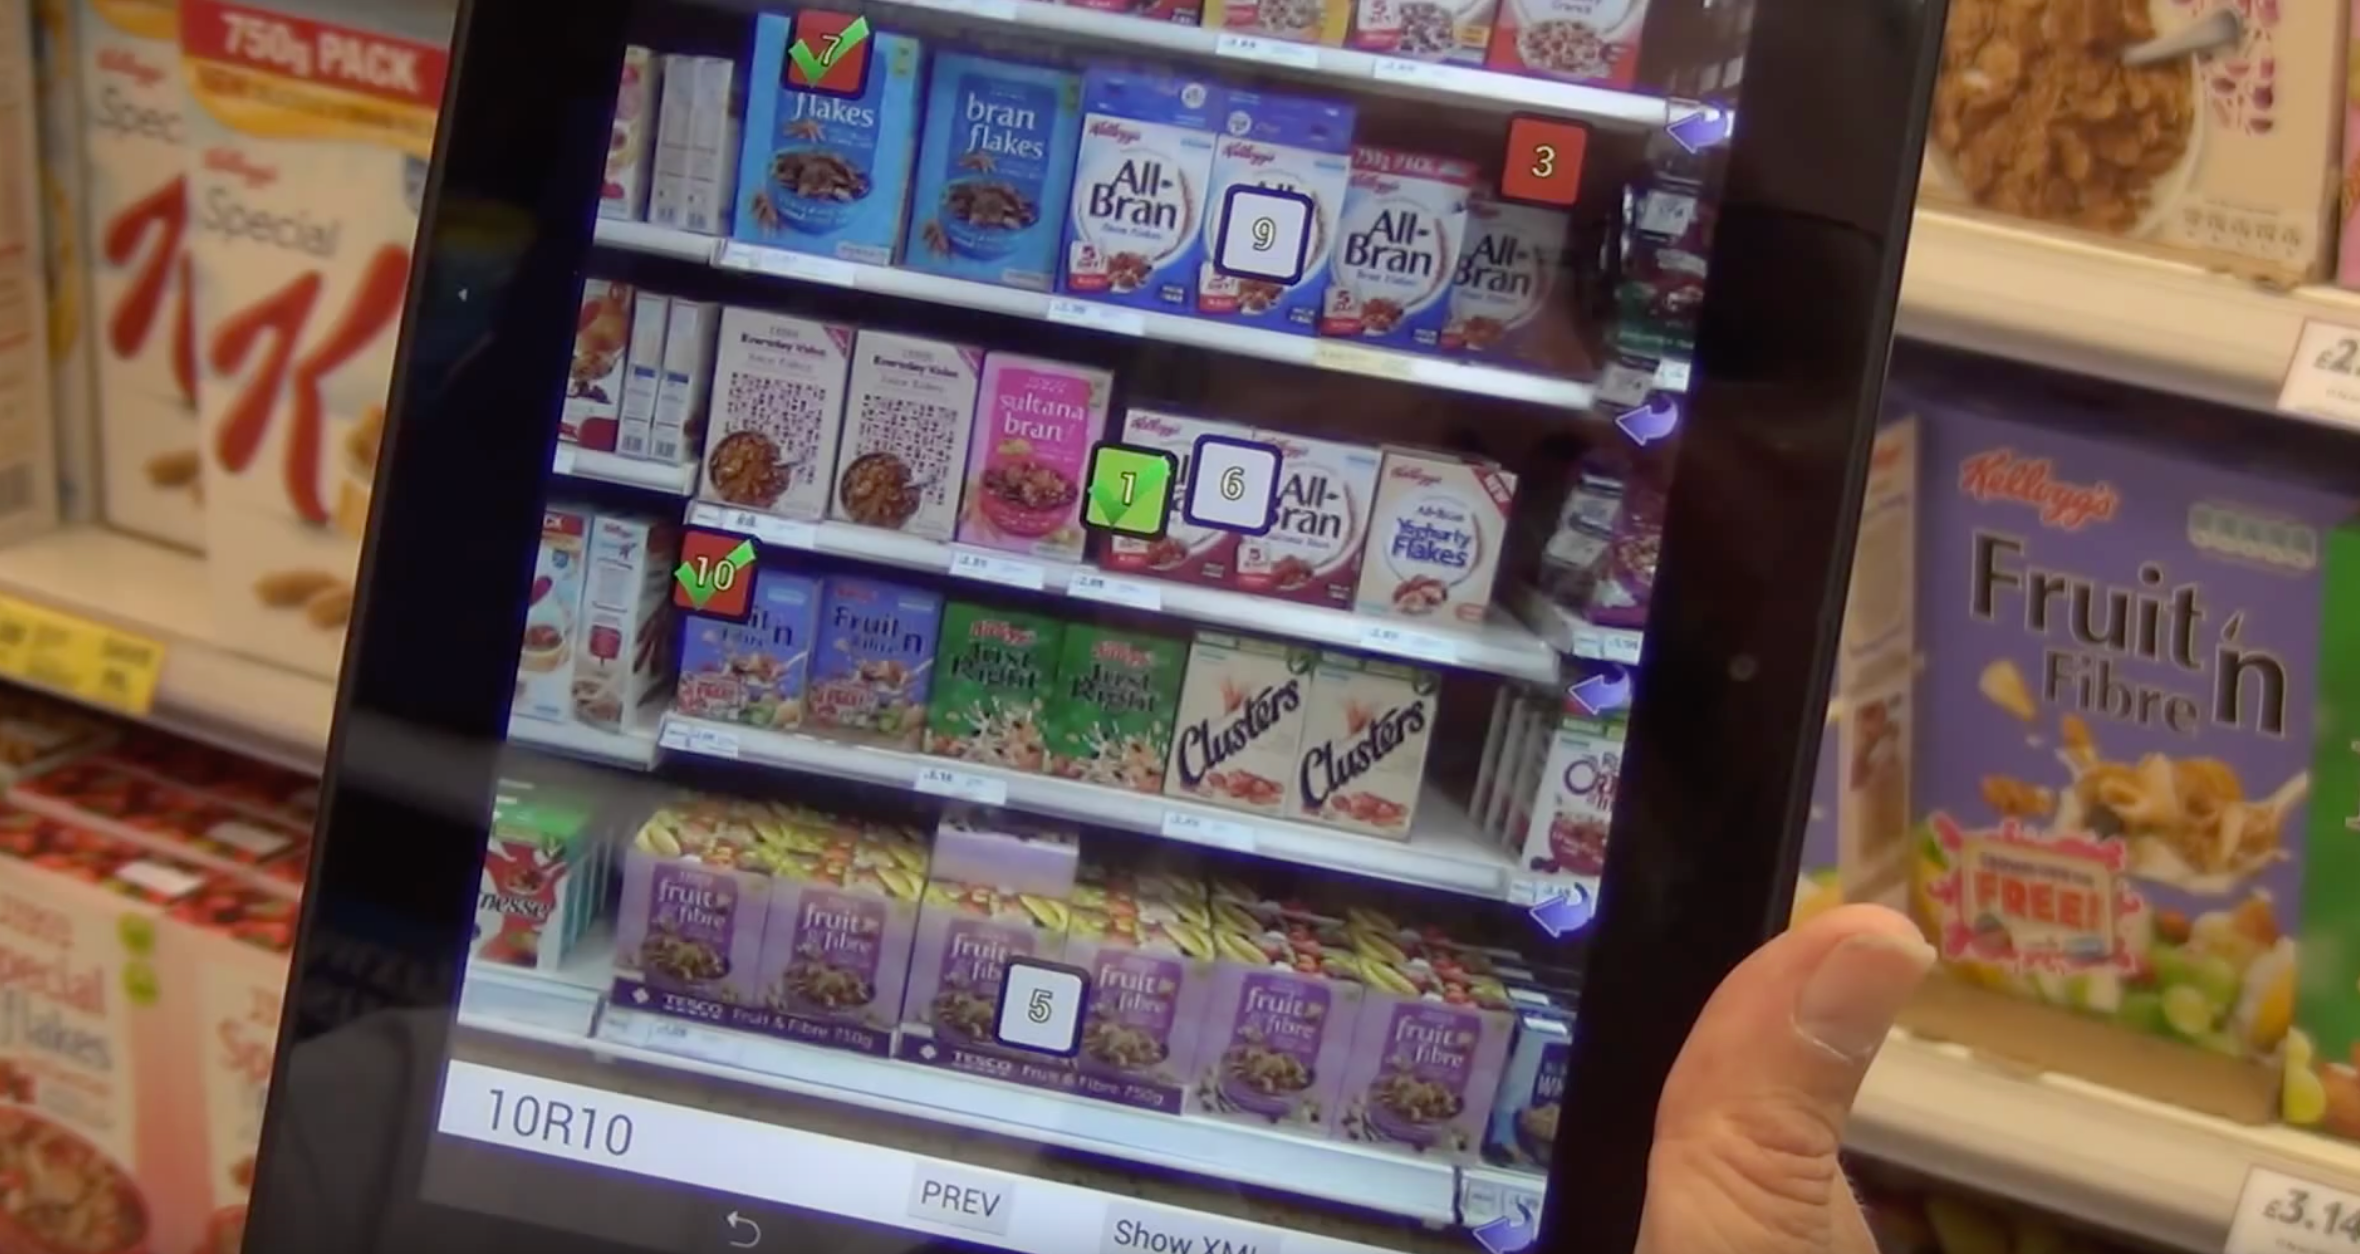
\includegraphics[scale=0.35]{Resources/Hintergrund/IBM.png}
		\caption[IBM Shopping App]{IBM Shopping App\footnotemark}	
	\end{center}
\end{figure}

\footnotetext{Quelle: \url{https://busy.org/@billigeplaetze/3waystodoaugmentedrealitywrong-3e0y2hze7f} vom 04.01.2019}

Auch IKEA nutzen die Möglichkeiten von AR in ihrer IKEA Place App zur Unterstützung bei Kaufentscheidungen. Die Applikation lässt den Nutzer Möbelstücke virtuell im physikalischen Raum positionieren. Er wählt ein Möbelstück aus dem Katalog und richtet seine Kamera auf die gewünschte Position dafür im Raum. Auf dem Display, zwischen den physikalischen Möbeln, erscheint nun ein virtuelles Modell des Möbelstücks in Originalgröße. Die Farben werden sogar an die Lichtverhältnisse angepasst. Der Nutzer kann das Möbelstück aus allen möglichen Blickwinkeln betrachten, wodurch er eine bessere Kaufentscheidung treffen kann und sich viel Zeit und Geld spart \cite{helander_joel_2017}.

\begin{figure}[h]
	\begin{center}
		\noindent\includegraphics[scale=0.4]{Resources/Hintergrund/ikea.jpg}
		\caption[IKEA Place App]{IKEA Place App\footnotemark}	
	\end{center}
\end{figure}

\footnotetext{Quelle: \url{https://mashable.com/2017/09/24/download-this-ikea-place-ar-kit-app/?europe=true##5LARqrPSqiqW} vom 04.01.2019}

Xiangyu Wang \cite{wang_using_2007} beschreibt in seiner Arbeit, wie man einen Bauleiter mit AR beim planen einer Baustelle unterstützen kann. Dieser kann mit der von Wang implementierten AR Applikation den gesamten Aufbau der Baustelle planen und visualisieren. 3D Objekte von Baustellenobjekten (siehe Abbildung \ref{bauModelle}), wie beispielsweise Kräne oder Bagger, können auf einer virtuellen Abbildung der Baustelle, welche der Nutzer vor sich z.B. auf einem Tisch angezeigt bekommt (siehe Abbildung \ref{baustelle}), positioniert werden. Auch Transport- und Fahrwege zeichnet er damit direkt in den Plan ein. Zusätzlich hat Wang bekannte Planungsregeln implementiert. Diese unterstützen den Bauleiter bei der Planung und helfen gleichzeitig bekannte Planungsfehler zu vermeiden, in dem diese auf dem Modell markiert werden. Laut Wang lässt sich mit seiner Applikation die Zeit für die Planung deutlich verringern, sowie die Qualität des Endprodukts steigern. Durch die Einhaltung der Planungsregeln lässt sich auch die benötigte Zeit für die Ausführung des Bauvorhabens verringern, da damit Adjustierungen des Plans während dem Bau vermieden werden können. Das vereinfacht die Arbeit besonders für Einsteiger und Laien. Durch die Visualisierung der Baustelle lässt sich der Plan auch leicht an die Arbeiter vermitteln und als Referenz nutzen, was Fehler bei der Ausführung vermeiden kann. Als weitere Funktionalität ist geplant sich diese Hologramme der Planung auch direkt auf der physikalischen Baustelle anzeigen zu lassen.

\begin{figure}[h]
	\begin{center}
		\noindent\includegraphics[scale=0.4]{Resources/Hintergrund/baustelle.png}
		\label{baustelle}
		\caption[AR Planner: Ansicht der Baustelle]{AR Planner: Ansicht der Baustelle\footnotemark}	
	\end{center}
\end{figure}

\footnotetext{Quelle: \cite{wang_using_2007}}

\begin{figure}[h]
	\begin{center}
		\noindent\includegraphics[scale=0.4]{Resources/Hintergrund/bauModelle.png}
		\label{bauModelle}
		\caption[AR Planner: 3D Modelle der Baumaschinen]{AR Planner: 3D Modelle der Baumaschinen\footnotemark}	
	\end{center}
\end{figure}

\footnotetext{Quelle: \cite{wang_using_2007}}

Das, in Sektion \ref{sec:label} beschriebene PaletteCAD Tool bietet auch Funktionalitäten für VR und AR an. Das Modell kann auf eine VR Brille übertragen werden, damit der Nutzer sich in diesem Raum bewegen kann und einen Eindruck davon bekommt. Für Tablets und Smartphones sind bereits AR Lösungen dazu implementiert. Dabei sieht man sich den Raum \enquote{durch die Smartphonekamera} an. Auf dem Display erscheinen die, per PaletteCAD positionierten Objekte. Der Raum muss davor exakt spezifiziert werden, damit die Hologramme an den richtigen Orten angezeigt werden können. Diese Funktionalität ist auch für Datenbrillen, wie die Microsoft HoloLens geplant.

AR als Visualisierungswerkzeug bringt einige Vorteile mit sich. Es unterstützt den Kunden dabei, sich das Endergebnis einer Arbeit vorzustellen, indem ihm das Ergebnis direkt im Raum gezeigt wird. Gleichzeitig erleichtert es so die Kommunikation zwischen Laien und Experten. Es kann deutlich am Plan gezeigt werden, wo Änderungen vorgenommen werden sollen. Teilweise kann durch AR auch Zeit und Geld gespart werden, da kein physikalischer Prototyp für einen Auftrag gebaut werden muss. Dieser kann einfach virtuell erstellt werden, wodurch er kein Material benötigt und beliebig verändert werden kann. Zusätzlich dient ein virtuelles Bild des Vorhabens der Orientierung bei der Arbeit. Das Modell ist im Vertrag verankert, wodurch die Arbeiter wissen worauf sie hinarbeiten und die zu bringende Leistung präzise dokumentiert ist.

Viele der oben gezeigten AR Applikationen existieren hauptsächlich für Tablets und Smartphones. Diese Geräte sind auch die Zugänglichsten, mit der größten Nutzergruppe. Eine kostenintensivere Lösung, welche in den letzten Jahren immer mehr an Aufmerksamkeit erlangt, sind Datenbrillen. Diese bieten den Vorteil gegenüber Handhelds, dass man bei ihrer Benutzung beide Hände frei hat, was sich besonders für Handwerker anbietet. Diese können in einer realen Umgebung mit Hologrammen interagieren, sich beispielsweise Beschreibungen anzeigen lassen und gleichzeitig an einer Maschine oder einem Problem arbeiten. Zusätzlich lassen Datenbrillen den Nutzer in seiner physikalischen Umgebung in die virtuelle Welt eintauchen. Die Hologramme werden um ihn herum angezeigt und verändern sich mit der Änderung seiner Blickfeldes. Das ermöglicht intuitive Interaktion und Bewegung im Raum, ohne gegen etwas zu laufen. Diese Bewegungsfreiheit ermöglicht es auch Pläne oder Modelle aus allen Richtungen zu betrachten und so besser zu verstehen. Der Nutzer betrachtet also nicht nur ein 3D Modell sondern \enquote{erlebt} es\cite{TODO:Buchkapitel}. Daher bieten Datenbrillen hohes Potential für das Handwerk und KMUs.
\chapter{Methoden}

Dieses Kapitel behandelt die in dieser Arbeit angewandten Methoden zur Erhebung der Daten und Erarbeitung der Lösung zu einem gefundenen Problem. Es soll die Vorgehensweise theoretisch beschreiben und untermauern.

\section{Fokusgruppe}
\label{sec:fokus}

Bei einer Fokusgruppe handelt es sich um ein moderiertes Diskursverfahren, bei dem ein Meinungsbild durch die Interaktion einer ausgewählten Gruppe erzeugt wird und somit Daten über ein festgelegtes Thema erhoben werden. Man kann es als Kombination aus fokussiertem Interview und Gruppendiskussion sehen. Als Instrument zur Datenerhebung in den Sozialwissenschaften hat es sich in den 60er und 70er Jahren etabliert. Es wird für folgende Felder verwendet \cite{schulz_quick_2012}:

\begin{itemize}
	\item Testverfahren
	\item Analyse an Meinungsvielfalt
	\item Instrument zur Akzeptanzanalyse
	\item Instrument zur Konfliktschlichtung
	\item Evaluierung bestimmter Maßnahmen
	\item Technikvorausschau
	\item Analyse heikler Aspekte aus dem Gesundheitsbereich
\end{itemize}

Normalerweise bestehen die Gruppen aus sechs bis zwölf Personen und einem Moderator. Die Gruppengröße kann jedoch auch erhöht werden, um eine bessere Repräsentanz zu erhalten. Alle Teilnehmer können je nach Ziel der Fokusgruppe zufällig oder nach Kriterien, wie Geschlecht, Lebensstil oder Beruf gewählt werden. Bestenfalls kennen sich die Teilnehmer untereinander nicht. \\
Der Moderator hat die Aufgabe den Dialog zwischen den Diskutierenden am laufen zu halten. Die Diskussion soll ein lebendiges Gespräch sein, welches von den Teilnehmern getragen und durch den Moderator, der sich an einem Leitfaden als Gedächtnisstütze orientiert, gelenkt wird. Er achtet auch darauf, dass Personen nicht durcheinander reden. Bohnsack und Schäffer legen vier Vorgehensweisen eines guten Moderators fest \cite{bohnsack_gruppendiskussionsverfahren_2001}:

\begin{itemize}
	\item Unterlassung inhaltlicher Stellungnahmen
	\item Ansprechen der gesamten Gruppe bei Interventionen
	\item Fragen nicht an Einzelne, sondern an das Kollektiv richten
	\item Vermeidung der Individualkommunikation von einzelnen Teilnehmern mit dem Moderator
\end{itemize}

Der Ablauf einer Fokusgruppe lässt sich in drei Phasen unterteilen \cite{schulz_quick_2012}. Die \textit{erste Phase} dient der inhaltlichen und organisatorischen Vorbereitung der Fokusgruppe. Der Moderator erstellt den Leitfaden und bestimmt und rekrutiert die Gruppe an Personen. Die Fokusgruppe leitet er dann mit einem Film, Bild, einer Homepage oder einem Vortrag ein, um den Teilnehmern das Thema näher zu bringen.\\
Die Diskussion stellt die \textit{zweite Phase} und die umfangreichste dar. Die Aufgabe des Moderators ist es dabei, das Gespräch anzuregen und dafür zu sorgen, dass jeder Teilnehmer einbezogen wird und aktiv an der Diskussion teilnimmt. Es ist für den Moderator von Vorteil einen Assistenten zu haben, der sich um kleinere Aufgaben und das Protokollieren der Erkenntnisse kümmert. Dies sollte schriftlich festgehalten werden und kann durch Audioaufzeichnungen und/oder Videoaufzeichnungen komplementiert werden. Videos sind dabei mit Vorsicht zu nutzen, da diese das Teilnahmeverhalten der Teilnehmer negativ beeinflussen können. \\
Das Meinungsspektrum der Gruppe ist dabei das interessante Ergebnis. In der \textit{dritten Phase}, der Datenanalyse und Interpretation der Ergebnisse müssen alle Aufzeichnungen, also schriftliche, Video- und Audioaufnahmen gemeinsam ausgewertet werden. So erhält man eine Sammlung an Meinungen der gesamten Gruppe, welche teilweise repräsentativ für ein bestimmtes Feld sind.

\section{Ethnographie: Teilnehmende Beobachtung}

\textit{``Will man etwas über andere Menschen herausfinden, \\
	geht man einfach zu ihnen hin, bleibt eine Weile, \\ 
	macht das mit, was diese Menschen dort normalerweise treiben, \\ 
	und lernt sie so durch eigene Erfahrung besser kennen.`` - Götz Bachmann} \cite{kuhl_handbuch_2009}

\subsection{Zusammensetzung der Methode}

Es sollen nun Ansatzpunkte gefunden werden, um die Theorie "Handwerker können durch den Einsatz von Technologie unterstützt werden und Zeit sparen" zu stärken. In der Ethnographie unterscheidet man dabei drei Varianten \cite{spittler_teilnehmende_2001}:

\begin{itemize}
	\item \textbf{Sammelzentriert:} Ethnographie unter der Prämisse, man muss und kann alle Informationen zu einem Gebiet sammeln.
	\item \textbf{Theoriezentriert:} Beobachtetes und Fakten werden "im Lichte einer Theorie" ausgewählt und geordnet. Hierzu zählt unter anderem die teilnehmende Beobachtung.
	\item \textbf{Problemzentriert:} Die Ethnographie stellt ein komplexes Problemfeld vor. Der Fokus liegt dabei nicht auf den Theorien des Forschers.
\end{itemize}

Diese Ethnographie fällt unter zweitere Kategorie, da die Aufzeichnungen genutzt werden, um oben genannte Theorie zu untersuchen. 

Im klassischen Sinne werden Sachverhalte durch Fragebögen und systematische Interviews beleuchtet. Mit diesen Methoden können zwar in kurzer Zeit viele Informationen erhoben werden, jedoch werden sie häufig als extrem künstlich kritisiert. Diese statische Atmosphäre kann dazu führen, dass kein gutes Gespräch zustande kommt und der Handwerker nur genau auf die Fragen antwortet und Informationen zurückbehält. Der Fakt, dass berufliches Wissen oft als Geheimnis angesehen und nur spärlich und selektiv weitergegeben wird, spielt hier noch negativ mit ein \cite{spittler_teilnehmende_2001}. Deshalb sollten Fragebogen und Interview für diese Forschung noch komplementiert werden.

Ein Blick fängt oft mehr ein als Worte. Deshalb wird zum Erheben der Informationen noch die Beobachtung der Arbeit eines Handwerkers hinzugefügt. Laut Spittler \cite{spittler_teilnehmende_2001} gibt es drei Prämissen, die eine Beobachtung, zusätzlich zu einem Interview befürworten:

\begin{enumerate}
	\item "Forschungspragmatisch besitzt die Beobachtung in manchen Situationen einen Vorteil gegenüber der Befragung."
	\item "Die sprachliche Erfassung stößt wegen Geheimhaltung, Schweigen und Verschweigen auf Schwierigkeiten."
	\item "Handlungen sind sprachlich gar nicht oder nur unter großen Schwierigkeiten erfassbar. (tacit knowledge)"
\end{enumerate}

Um die Arbeit eines Handwerkers besser zu verstehen, reicht es nicht sich diese nur von ihm Beschreiben zu lassen. Bei der Ausübung seines Handwerks kann er keine Schritte "verschweigen" und der Forscher kann diese direkt analysieren. Indem er sein Notizheft beiseite legt und selbst mitarbeitet, kann er sich ein genaues Bild des Handwerks machen und so auch kleine Ansatzpunkte zum bekräftigen seiner Theorie finden \cite{malinowski_argonauts_1922}. Deshalb wurde die Teilnehmende Beobachtung als Methode der Ethnographie gewählt.

\subsection{Beschreibung der Methode}

Feldforschung ist eine der ältesten und am weitesten verbreiteten Techniken zur Datenerhebung in einem unbekannten Forschungsgebiet. Die Forschungspraxis hängt dabei in hohem Maße von der \textit{Persönlichkeit der Forschers}, der \textit{Beschaffenheit des Feldes} und der \textit{Interaktion des Forschers mit dem Feld} ab. Das bedeutet die Forschung lässt sich schlecht genau durchplanen und der Forscher kann sie nur begrenzt kontrollieren. Einige Ethnologen argumentieren, dass gerade das den Reiz der Methode ausmacht \cite{rottenburg_feldforschung_nodate}. Andere bezeichnen die teilnehmende Beobachtung deshalb als "methodenfeindlich" \cite{kuhl_handbuch_2009}. Daraus geht hervor, dass es keinen besten Weg gibt diese Methode durchzuführen, nur Anregungen und Tipps.

Zur Datenerhebung sind die Punkte \textit{Forschungsanfang}, \textit{Rollenzuweisung}, \textit{Beobachtungsdauer}, \textit{wo und wie beobachtet wird}, sowie das \textit{Aufschreiben der Erlebnisse} zu beachten \cite{kuhl_handbuch_2009}. Diese werden im Folgenden erläutert. \\
Der erste Tag im Feld ist laut Bachmann einer der anstrengendsten. Nicht nur Beobachten und die ersten Eindrücke verarbeiten, muss der Forscher an diesem Tag, es kommen auch einige soziale Aufgaben auf ihn zu. Er muss die neuen Kollegen in seinem Forschungsumfeld kennenlernen, sowie überlegen, wie er sich diesen gegenüber gibt. Am besten sollte er sich neutral präsentieren und sich nicht verstellen, um ein nettes Verhältnis den zu Erforschenden gegenüber aufzubauen. Das erzeugt gegenseitiges Vertrauen. Trotzdem sind seine Eindrücke in den ersten Tagen dadurch getrübt. \\
Meist schlüpft der Forscher hierbei in die Rolle des Praktikanten, der nicht viel kann, viel nachfragt und viel herumkommt. Andere Ansätze erwähnen auch die Rollen Auszubildender, Lehrling oder Trainee, welche jedoch weniger flexibel sind und dem Forscher eine geringere Bewegungsfreiheit bieten. \\
Im klassischen Sinne wurde eine Ethnographie über einen langen Zeitraum von ca. einem Jahr durchgeführt, was beispielsweise bei der Untersuchung des Arbeitsalltags auf einem Bauernhof Sinn ergab, jedoch in der modernen Forschung kaum mehr tragbar ist. Nun ist eine Dauer von zwei bis sechs Monaten üblich. Auch Zeiträume von einem Tag bis zu ein oder zwei Wochen können schon wertvolle Ergebnisse liefern, wecken jedoch Skepsis bei einigen Ethnologen. \\
Während der Arbeit beobachtet der Forscher kleine Details, die eventuell bei Gesprächen übergangen, oder nicht ausreichend wörtlich wiedergegeben werden können. Pausen, sowie die Zeit vor und nach der Arbeit, also Daten aus informellen Situationen, werden von einigen Forschern als sehr wichtig angesehen, da sie dem Forscher die Möglichkeit bieten sich mit den Erforschten auszutauschen und neue Kontakte zu knüpfen, über die er wieder neue Erkenntnisse oder Einblicke erlangen kann. Wie er an die besten Daten bekommt ist jedoch immer forschungsabhängig. Organisationsforscher legen dabei mehr Wert auf die Beobachtung der Arbeit. Graaf und Rottenburg \cite{rottenburg_feldforschung_nodate} sprechen hier von "dabeistehender Beobachtung", welche der Forscher ausführt, da er selbst wahrscheinlich nicht die Fähigkeiten besitzt, um die Tätigkeit selbst auszuführen. Er konzentriert sich also auf das Beobachten, Fragen stellen und führt eventuell Hilfstätigkeiten aus. Um spezielle Informationen zu erlangen, kann sich der Ethnologe auf \textit{Konflikte} konzentrieren, welche viel über die Organisation und die involvierten Personen aussagen. Ein anderer Ansatz ist, in "Anbedacht des Unbedeutenden" sein gesamtes Augenmerk auf eine kleine Bagatelle zu richten. Außerdem kann der Forscher einmalige, kleine Situationen herausgreifen und diese anhand des Kontexts und seines erworbenen Wissens analysieren. \\
Um das Wissen festzuhalten, macht sich der Ethnologe am besten direkt nach einem Sachverhalt Notizen für später, als Erinnerungsstütze. Das hilft ihm beim zweiten Schritt, dem Ausformulieren in einem Forschungstagebuch. Dabei kann er entweder das erlebte sachlich und in der Ausführung präzise beschreiben, oder bereits beim Ausformulieren seine Interpretationen einfließen lassen. Auch das ist wieder abhängig von der betriebenen Forschung. Er sollte sich von Anfang an einen Zitierstil zum kennzeichnen von verschiedenen Zitaten in unterschiedlichen Kontexten aneignen und konsequent durchziehen. Zusätzlich zum Forschungstagebuch kann der Ethnologe ein Tagebuch für \textit{persönliche Gefühle und Erfahrungen}, \textit{Ideen und theoretische Erwägungen} und/oder einen \textit{Forschungskalender}, in den er seine nächsten Schritte einträgt, führen. Oft reicht die Zeit nach Feierabend nicht aus, um alle Erlebnisse nachzutragen, weshalb es auch sinnvoll sein kann sich unter Tags Zeit und einen Platz zum Arbeiten zu schaffen. 

Mit dieser Methode lässt sich ein Beruf analysieren, wobei man nicht alle Einzelheiten festhalten kann. Dadurch ist es dem Forscher möglich Ansatzpunkte für weitere Forschung oder Verbesserungen zu finden.

\section{Gestaltungsorientierte Forschung: Implementieren eines Prototypen}
\label{sec:gestForsch}

Mit den Methoden Fokusgruppe und Ethnographie wird ein bestehendes Problem genauer beleuchtet und dabei herausgearbeitet, ob die Lösung dieses Problems wünschenswert ist. Auf Basis des erörterten Umstands soll dann eine Lösung gefunden werden, die dem Forscher und allen beteiligten Parteien genügt. Dabei stellt sich die Frage, wie man das Problem adressiert. Für problembasierte Forschung ist der Weg zu einer Lösung nicht geradlinig, weshalb ein flexibler Ansatz genutzt werden soll, wofür sich laut Hevner et al. \cite{hevner_design_nodate} die Methode \textit{Gestaltungsorientierte Forschung} anbietet. Dabei wird von einem Problem augegangen und über einen inkrementellen, iterativen Prozess eine Lösung erarbeitet. Hevner identifiziert dazu fünf charakteristische Faktoren von Problemen, die mit gestaltungsorientierter Forschung angegangen werden \cite{hevner_design_nodate}:

\begin{enumerate}
	\item ``Environmental factors such as requirements and constraints are poorly defined"
	\item ``An inherent complexity in the problem and possible solutions"
	\item ``A flexibility and potential for change of possible solutions"
	\item ``A solution at least partially dependent on human creativity"
	\item ``A solution at least partially dependent on collaborative effort"
\end{enumerate}

Das Erfüllen dieser Kriterien qualifiziert ein Problem für gestaltungsorientierte Forschung. Basierend auf den Arbeiten von Hevner und anderen renommierten Wissenschaftlern entwickelte Pfeffers ein \textit{6-Phasen Modell} zur Durchführung einer solchen Forschung \cite{j._ellis_guide_2010}. Dabei werden die Phasen \textit{Problemidentifikation und Motivation} zur Begründung der Forschung, \textit{Ziel der Lösung}, \textit{Gestaltung und Entwicklung}, sowie \textit{Demonstration des Artefakts}, \textit{Evaluation} der Tests und \textit{Kommunikation der Ergebnisse} durchlaufen \cite{peffers_design_2007}. 

\begin{figure}[h]
	\begin{center}
		\noindent\includegraphics[width=\linewidth,height=\textheight,keepaspectratio]{Resources/DS_Peffers.png}
		\caption{Peffers et al.: Gestaltungsorientierte Forschung \cite{peffers_design_2007}}
	\end{center}
\end{figure}

Diese sechs Phasen können sequentiell von der ersten bis zur letzten durchgearbeitet werden, aber nicht zwangsläufig. Ein Forscher kann auch an einer für ihn passend erscheinenden Phase beginnen und von dort aus weiterarbeiten. Problemzentrierte Forschung beginnt in Phase 1, \textit{Problemidentifikation und Motivation}. Dieser Ansatz wird häufig gewählt, wenn auf früherer Forschung aufgebaut oder von der Beobachtung eines Problems begonnen wird. Zielorientierte Forschung hingegen startet meistens in Phase 2, \textit{Ziel der Lösung}. Dies wird oft durch einen Anstoß aus der Industrie angetrieben. Gestaltungsorientierte Ansätze beginnen mit Phase 3, \textit{Gestaltung und Entwicklung}. Dabei gehen die Forscher meist von einem unfertigen, nicht komplett durchdachten Artefakt aus früherer Forschung oder Projekten aus. Eventuell stammt das Artefakt sogar aus einer anderen Forschungsdomäne und wurde zur Lösung eines anderen Problems erstellt. Mit Phase 4, \textit{Demonstration des Artefakts} beginnt die kunden- oder kontextbasierte Forschung. Dabei entstand die Idee beim Beobachten einer praktischen Lösung, welche funktioniert. Die Forscher arbeiten dabei rückwärts und versuchen so die bestehende Lösung zu verbessern. Dieser Ansatz kann aus einer Consultingerfahrung hervorgehen.

In dieser Arbeit wird mit Phase 1 begonnen, da das Problem anfangs durch die Ethnographie identifiziert wurde. Im Folgenden wird die Methode von Peffers genauer beschrieben \cite{peffers_design_2007}.

\subsection{Problemidentifikation und Motivation}

Peffers diskutiert Ansätze verschiedener Wissenschaftler zu Problemidentifikation und wie man Ideen findet, welche umsetzenswert sind. Der Ansatz, welcher von Pfeffers aufgegriffen wird, von Archer \cite{archer_systematic_1965} und Eekels \cite{eekels_methodological_1991} bezieht sich auf angewandte Probleme, also welche die bei einer Tätigkeit auffallen, auftreten und behindern. \\
In diesem Abschnitt muss die Suche nach einer Lösung für ein Problem begründet werden. Der zu betrachtende Umstand wird dafür genau dargelegt und definiert. Das Problem wird in kleine Teile gespalten und genau beleuchtet. Durch eingehende Betrachtung kleiner Teilbereiche kann die Komplexität des Problems in der Lösung abgebildet werden. Nur aus einer ausreichenden Problembeschreibung lässt sich ein fundiertes Artefakt erzeugen. 

Aus der Motivation ergeben sich zwei Vorteile für den Forscher: \\
Das Problem zu identifizieren und so die Suche nach einer Lösung zu begründen motiviert den Forscher, sowie die Leser seiner Arbeit bei der Suche und der Akzeptanz der Ergebnisse. \\
Zusätzlich hilft es Lesern seine Schlussfolgerungen nachzuvollziehen. \\
Um diesen Schritt durchzuführen stehen das Wissen über den aktuellen Stand des Problems, sowie die Wichtigkeit der Lösung als Ressourcen zur Verfügung. Daraus lassen sich die Anforderungen an eine Lösung zusammenstellen \cite{peffers_design_2007}.

\subsection{Ziel der Lösung}

Auch wenn das Problem gut spezifiziert ist, lässt es sich oft nicht direkt in Ziele übersetzen. Diese lassen sich besser über einen inkrementellen Prozess bestimmen, als direkt festlegen. Damit sollen die performance Ziele der Lösung herausgearbeitet werden. 

Grundlegend leitet man die Ziele von der Problemdefinition, sowie dem Wissen was möglich und machbar ist ab. Dabei kann das Ziel quantitativ sein, also beispielsweise Umstände darlegen, für welche die angestrebte Lösung besser ist als eine existierende. Oder es handelt sich um ein qualitatives Ziel, bei dem ein Artefakt Lösungen oder Hilfe für Probleme bereitstellt, welche über das ursprüngliche Problem hinausgehen. Besonders wichtig ist dabei, dass alle Ziele logisch aus der Problemspezifikation herleitbar sind. Als Ressource zur Herleitung der Ziele sollte der aktuelle Stand des Problems, als auch bereits verfügbarer Lösungen (falls existent), vorhanden sein und deren Zweckmäßigkeit überprüft werden.

\subsection{Gestaltung und Entwicklung}

Aus den gefundenen Problemen und Zielen wird nun ein Artefakt entwickelt. Für Peffers Gestaltungsorientierte Forschung kann man dabei nach dem Prinzip "early prototyping" vorgehen, da es sich um einen inkrementellen Prozess handelt. Alle Wissenschaftler, welche Peffers untersuchte legten den Fokus auf diese Phase.

Es wird dabei ein Artefakt erzeugt. Artefakte sind für Peffers Konstrukte, Modelle, Methoden, Instantiierungen oder "new properties of technical, social, and/or informational resources" \cite{jarvinen_action_2007}. Generell ist dabei jedes Forschungsartefakt ein Objekt, welches durch Zuhilfenahme von wissenschaftlichen Beiträgen entstanden ist. Dies beinhaltet die Funktion und die Architektur des Artefakts festzulegen und daraus dann das Artefakt zu kreieren. Dabei soll der Wissenschaftler theoretisches Wissen als Ressource nutzen, welches in der Lösung zum tragen kommen soll.

\subsection{Demonstration des Artefakts}

Um die Funktionstauglichkeit des Artefakts zu testen wird es vorgezeigt. Dabei kann entweder ein Test stattfinden, um zu zeigen, dass die Idee funktioniert, oder mehrere Tests, um eine genauere Evaluation durchzuführen.

Das Artefakt wird dabei so vorgeführt, damit deutlich wird, dass es eins oder mehr der anfangs definierten Probleme lösen kann. Dazu zählt die Verwendung des Artefakts in Experimenten, Simulationen, Case Studies, Beweisen oder anderen geeigneten Aktivitäten. Als Ressource zum Durchführen der Demonstrationsphase gilt das Wissen, wie man das Artefakt einsetzen muss, um ein Problem zu lösen.

\subsection{Evaluation}

Das Artefakt wurde untersucht und nun müssen die Informationen verwertet werden. Dazu ist wichtig, dass vor der Demonstration Werte festgelegt werden, welche dabei erfasst werden. Der Wissenschaftler muss genau beobachten und messen, wie gut das Artefakt die Lösung des Problems unterstützt. Dazu vergleicht er die Ziele der Lösung mit den tatsächlich beobachteten Ergebnissen der Demonstration des Artefakts. Um dies erfolgversprechend durchzuführen, wird ein Wissen über relevante Metriken und Analysetechniken verlangt.

Der Charakter der Forschung entscheidet dabei, welche Form der Evaluation durchgeführt wird. Dabei werden Methoden verwendet, wie beispielsweise das Vergleichen der Artefaktfunktionalität mit den Zielen der Lösung aus Phase 2, quantitative Leistungsmesswerte, wie hergestellte Güter oder erwirtschaftetes Kapital, Ergebnisse von Zufriedenheitsumfragen, Kundenfeedback, Simulationen, oder quantifizierbare Messwerte der Systemperformanz, wie Reaktionszeit oder Verfügbarkeit des Systems. Die Evaluation kann alle möglichen geeigneten empirischen Daten oder logische Beweise enthalten.

Am Ende dieser Phase kann der Forscher entscheiden ob er wieder zu Phase 3 zurückgeht und die gewonnenen Erkenntnisse nutzt um ein neues, besseres Artefakt zu entwickeln, oder ob er in die letzte Phase der Methode fortschreitet und die weitere Entwicklung zukünftigen Projekten überlässt. Dabei gibt die Art der Forschung an, welche Methode sinnvoller ist.

\subsection{Kommunikation der Ergebnisse}

Die gewonnenen Erkenntnisse müssen nun entsprechend Kommuniziert werden, um sie zu verbreiten. Dies sollte das Problem und seine Wichtigkeit, das Artefakt und seine Nützlichkeit und Neuartigkeit, die Einzelheiten des Designs und seine Effektivität enthalten. Die Publikation sollte an andere Wissenschaftler oder relevante Gruppen, wie zum Beispiel praktizierende Personen aus dem entsprechenden Bereich gerichtet sein. 

In wissenschaftlichen Publikationen kann die Struktur dieser Methode genutzt werden, um die Ausarbeitung zu strukturieren, wie beispielsweise empirische Forschung durch den empirischen Prozess (Problemdefinition, Literaturrecherche, Aufstellen der Hypothesen, Datensammlung, Analyse, Ergebnis und Fazit) strukturiert wird. Die Kommunikation der Ergebnisse erfordert Wissen darüber, wie Arbeiten in der entsprechenden Disziplin verfasst werden. 

\section{Design des Fragebogens}

Diese Arbeit zielt darauf ab, einen theoretischen, sowie einen praktischen Beitrag abzuleiten. Dazu wurden Anmerkungen der Testpersonen während und nach den Probandentests notiert. Diese Informationen können dazu genutzt werden, Ideen zu sammeln und die Applikation zu verbessern, allerdings lassen sie sich nicht gut vergleichen. Sie stellen den praktischen Beitrag dar. Für den theoretischen Teil benötigt man vergleichbare Werte und Größen. Dazu wurde ein Evaluationsbogen konzipiert, der folgende Fragen beantworten soll:

\begin{itemize}
	\item Wie ist der Bezug des Handwerkers zu technischen Geräten?
	\item Wie komplex ist der Umgang mit dem System?
	\item Kann der Handwerker sich vorstellen die Technologie in Zukunft zu nutzen?
\end{itemize}

Ersteres soll Helfen abzuschätzen, wie sehr die technische Versiertheit des Handwerkers sich auf die Akzeptanz bzw. das Interesse an der Applikation auswirkt. \\
Die Nutzung eines neuen Systems, in diesem Fall einer AR Anwendung, stellt für die Handwerker aus unternehmerischer Sicht eine Risiko dar. Deshalb ist es essentiell bestimmen zu können, ob die Anwendung von den Nutzern akzeptiert und genutzt werden wird. Die beiden weiteren Fragen sollen Aufschluss darüber geben, wie die Einstellung der Fachkräfte zu dieser neuen Technologie ist. Um diese Fragen zu beantworten, werden psychologisch und wirtschaftlich evaluierte Modelle verwendet. 

Um die Gebrauchstauglichkeit der Applikation zu testen, wird das \textbf{SUS} (System Usability Scale) \cite{brooke_sus_nodate} Modell verwendet. Es gibt Aufschluss darüber, wie einfach oder umständlich die Bedienung für den Handwerker war. \\
Ein System wird nicht genutzt, wenn der Nutzer die Interaktion damit als zu Anstrengend empfindet. Um herauszufinden, als wie fordernd der Handwerker die Nutzung der Applikation empfindet, wird das Modell \textbf{NASA-TLX} verwendet. \\
Zusätzlich werden noch \textbf{TAM} und \textbf{TAM2} angewandt. Diese Abkürzungen stehen für Technology Acceptance Model. Sie wurden entwickelt, um vorherzusagen, wie wahrscheinlich ein Anwender eine Technologie nutzen wird. \\
Im folgenden werden die Modelle erklärt.

\subsection{SUS}

Bei der \textbf{System Usability Scale} handelt es sich um einen einfachen, aus zehn Punkten bestehenden Fragebogen zur subjektiven Einschätzung der Gebrauchstauglichkeit eines Systems. Es ist eine \textbf{Likert Skala}, auf welcher die Zustimmung oder Ablehnung durch sieben Punkte angegeben werden kann. Sie hilft Aufschluss darauf zu geben, ob ein System benutzt werden wird, oder nicht. \\
Nach ISO 9241-11 sollte die Messung der Gebrauchstauglichkeit folgende Aspekte abdecken \cite{brooke_sus_nodate}:

\begin{itemize}
	\item \textit{Effektivität:} Die Fähigkeit des Nutzers gestellte Aufgaben mit Hilfe des Systems zu erledigen und die Qualität der Resultate.
	\item \textit{Effizienz:} Die Menge der konsumierten Ressourcen, nötig zur Erledigung der Aufgabe.
	\item \textit{Befriedigung:} Die subjektiven Reaktionen des Nutzers auf die Verwendung des Systems.
\end{itemize}

Diese Größen zieht auch der industrielle Nutzer in Betracht, wenn er über die Implementierung einer neuen Technologie in seinem Arbeitsalltag nachdenkt. Aus unternehmerischer Sicht ist es jedoch oft nicht rentabel, eine komplette Kontextanalyse durchzuführen. SUS, mit seinen zehn Fragen, liefert eine genügende Einschätzung der Abdeckung dieser Größen.

Zur Erstellung des Fragebogens wurde ein Katalog von 50 Fragen durch John Brooke und sein Team analysiert. Dabei haben sie die zehn Fragen herausgearbeitet, welche die stärksten zustimmenden bzw. ablehnenden Reaktionen bei Probanden hervorgerufen haben. Durch die erhaltenen subjektiven Antworten auf diese Fragen lässt sich abschätzen, wie viel Training und Unterstützung neue Nutzer des Systems brauchen werden, um dieses erfolgreich zu benutzen, und wie komplex es den Anwendern erscheint.

Laut John Brooke \cite{brooke_sus_nodate} sollen die Probanden den Fragebogen ausfüllen, nachdem sie das System getestet haben und bevor eine anschließende Diskussion beginnt. Dabei sollen diese ankreuzen, was ihnen ihr Gefühl nach dem Lesen der Frage sagt und nicht lang über diese nachdenken. Alle Fragen müssen dabei beantwortet werden. Sollte ein Proband auf eine Frage keine Antwort geben wollen oder können, wird das neutrale Ergebnis der Frage angekreuzt. \\
Einzelne Antworten auf Fragen sind alleine nicht aussagekräftig. Die gesamte Auswertung aller Antworten gibt jedoch einen Wert zwischen 0 und 100, welcher die generelle Gebrauchstauglichkeit der Applikation angibt.

\subsection{NASA-TLX}

Der von NASA entwickelte \textbf{Task Load Index} (NASA-TLX) ist ein weit verbreitetes Instrument zur Bestimmung der Beanspruchung eines Probanden bei einem Testszenario oder dem Testen einer Anwendung \cite{giesa_bewertung_2003}. Er wurde ausgewählt, um zu bestimmen, als wie Anstrengend Handwerker die Nutzung von Augmented Reality empfinden und ob das eine Auswirkung auf die Akzeptanz der Technologie, sowie der Anwendung hat. Dabei misst der Index die Beanspruchung in sechs Dimensionen:

\begin{itemize}
	\item Geistige Anforderungen
	\item Körperliche Anforderungen
	\item Zeitliche Anforderungen
	\item Leistung
	\item Anstrengung
	\item Frustrationsniveau
\end{itemize}

Diese lassen sich wiederum in drei Subskalen unterteilen \cite{gros_bestimmung_2004}:

\begin{itemize}
	\item Merkmale der Aufgabe: geistige, körperliche, zeitliche Anforderungen
	\item Verhaltensmerkmale: Leistung und Anstrengung
	\item Individuelle Merkmale: Frustration
\end{itemize}

Jede dieser Dimensionen wird auf einer Skala mit 20 Stufen angegeben, die jeweils von \textit{gering} bis \textit{hoch} reicht. Jede Stufe auf der Skala wird mit 5 Punkten gewichtet. Dadurch reicht jede von 0 bis 100 und gibt somit die erfahrene Belastung zu jeder Dimension in Prozent an. Zur Auswertung wird der ungewichtete NASA-TLX verwendet. Dabei werden alle Punkte zusammengezählt und durch die Anzahl der Dimensionen geteilt. Dabei erhält man wieder einen Wert zwischen 0 und 100.

Die originale Version des NASA-TLX sieht eine Gewichtung der einzelnen Dimensionen vor. Dieses Vorgehen wurde jedoch häufig kritisiert. Nygren \cite{nygren_psychometric_1991} schlägt vor ganz auf die Gewichtung zu verzichten. Pfendler \cite{pfendler_vergleichende_1991} gibt bei der deutschen Version des NASA-TLX an, dass durch Weglassen der Gewichtung des Gesamtwerts eine höhere Reliabilität erzielt werden kann. Deshalb wird auch hier auf die Gewichtung verzichtet.

Auch wenn der NASA-TLX hoch etabliert, diagnostisch und valide ist, wird doch erwähnt, dass die deutsche Version scheinbar weniger sensitiv ist als die englische \cite{horold_faktor_2015}. In dieser Arbeit wird die deutsche Version verwendet, da die App mit deutschsprachigen Probanden getestet wird. Es wird darauf vertraut, dass die Sensitivität ausreichend ist. 

Der Fragebogen wurde mit \LaTeX  aus dieser Vorlage erstellt \cite{https://doi.org/10.13140/rg.2.2.26978.79044}.

\subsection{TAM und TAM2}

Eines der am weitesten verbreiteten Modelle in der Akzeptanzforschung ist das \textbf{Technology Acceptance Model} (TAM) von Davis \cite{davis_perceived_1989}. Es ist aus der \textbf{Theory of Reasoned Action} (TRA) von Fishbein und Ajzen \cite{fishbein_belief_1975} und der darauf basierenden \textbf{Theory of Planned Behaviour} (TPB) von Ajzen \cite{ajzen_theory_1991} entstanden. Beide Modelle stammen aus der Psychologie und analysieren wie die Einstellung einer Person zu einer Handlung, sowie subjektive Normen das Verhalten dieser Person beeinflussen. TPB zieht zusätzlich den subjektiven Aufwand, zum bewältigen einer Handlung in Erwägung und erweitert so TRA. 

Davis schlug das TAM 1989 in seiner Dissertationsschrift vor. Es bietet, vor allem im industriellen Bereich, auf Basis der Nutzungsintention eine Möglichkeit die Akzeptanz einer nicht marktreifen Technologie zu prognostizieren \cite{wilhelm_nutzerakzeptanz_nodate}. Dabei kombiniert das TAM die Größen \textit{wahrgenommener Nutzen} und \textit{wahrgenommene Einfachheit der Nutzung}, um diese Aussagen zu treffen. Ersteres gibt an, ob der Nutzer sich eine Steigerung seiner Produktivität aus der Verwendung der Technologie verspricht. Zweiteres beschreibt für wie komplex der Nutzer die Anwendung der Technologie hält. Laut Davis bewegen diese beiden Faktoren Unternehmer dazu die Technologie zu verwenden und Mitarbeiter im Umgang damit zu schulen. Das TAM bietet zusätzlich eine hohe Flexibilität, wurde in zahlreichen Studien getestet und seine Aussagekraft bestätigt \cite{university_of_arkansas_dead_2007}.

Davis erweiterte sein Modell auf die Version TAM2, um mehr auf die wahrgenommene Nützlichkeit einzugehen. Seiner Meinung nach gibt diese Determinante großen Aufschluss über die Intention eines Nutzers, wurde aber bis zu dem Zeitpunkt nicht eindringlich betrachtet \cite{venkatesh_model_1996}. Dazu ergänzte er Einflussfaktoren auf das Konstrukt wahrgenommene Nützlichkeit um \textbf{soziale} und \textbf{-	Kognitiv-instrumentelle Prozessvariablen}, sowie Betrachtungen zu unterschiedlichen Messzeiten. Soziale Variablen beschreiben dabei den Einfluss der Umgebung einer Person auf ihr Verhalten. Also wie sieht das Umfeld der Person die getestete Technologie und welchen Einfluss hat das auf die Entscheidung der Testperson. Zweitere Variable gibt wiederum an wie relevant das Ergebnis durch die Nutzung der Technologie für die Arbeit des Nutzers ist und wie gut es sich präsentieren lässt \cite{venkatesh_theoretical_2000}. Studien belegen, dass soziale Prozessvariablen anfangs die wahrgenomme Nützlichkeit für Nutzer stark beeinflussen, dies jedoch abnimmt, sobald der Proband mehr Erfahrung gesammelt hat \cite{galli_technologieakzeptanz_2016}.

\begin{figure}[h]
\begin{center}
\noindent\includegraphics[width=\linewidth,height=\textheight,keepaspectratio]{Resources/TAM.png}
\caption{Technology Acceptance Modell}
\end{center}
\end{figure}




\chapter{Fokusgruppe}

In dieser Fokusgruppe wurde untersucht, wie Datenbrillen von Handwerkern aufgenommen werden und ob diese sich Szenarien vorstellen können, in welchen der Einsatz von Datenbrillen in ihrem Arbeitsumfeld hilfreich ist. Die Ursprüngliche Idee war dabei, dass Datenbrillen zur Unterstützung von Handwerkern eingesetzt werden, beispielsweise in Fernwartungsszenarien, wenn eine Person sehen möchte, was eine andere Person sieht, sich diese aber nicht am selben Ort befinden. Dann kann das Bild von der Brille des einen, zum Monitor des anderen übertragen werden. \\
Im Folgenden werden dazu die Rahmenbedingungen und die Intention, die Durchführung, sowie die Auswertung der geäußerten Ideen beschrieben. Dabei kristallisierten sich zwei Anwendungsbereiche für AR heraus, die genauer beleuchtet werden, da sie zum weiteren Verlauf dieser Forschung beitragen.

\section{Rahmen}

Um ein generelles Bild der Akzeptanz von Augmented Reality im Handwerk zu prüfen, wurde eine Fokusgruppe dazu in der Handwerkskammer München organisiert. Dazu wurden ca. 20 Handwerker aus verschiedenen handwerklichen Branchen eingeladen, um über das Thema zu diskutieren. Anfangs hielt der Moderator einen Vortrag über Augmented Reality allgemein, um den Teilnehmern die Technologie näher zu bringen. Anschließend standen verschiedene Datenbrillen, wie zum Beispiel Google Glass und die Microsoft HoloLens, zur Verfügung, welche von den Teilnehmern ausprobiert werden konnten. Die Forschungsfragen für den Workshop waren: "Was denken Handwerker über Augmented Reality, speziell Datenbrillen?" und "Können sich Handwerker Szenarien vorstellen, für welche der Einsatz von Datenbrillen für sie sinnvoll wäre?". Diese gab der Moderator den Testpersonen mit für das Testen der Brillen.

\section{Testen der Brillen}

Für jede Brille wurde eine eigene Station aufgebaut. Das Augenmerk dieser Arbeit liegt auf der Microsoft HoloLens, da dieses die am weitesten fortgeschrittene Technologie ist. Es handelt sich dabei um eine große Brille, welche mit Kameras, die ihre Umgebung filmt, sowie Mikrofon und Lautsprechern ausgestattet ist. Sie erlaubt es im Sichtfeld des Nutzers Hologramme anzuzeigen und mit diesen zu interagieren. Dieser sieht dabei die "reale Welt", welche durch die Hologramme erweitert wird. In der Fachliteratur wird dies als \textbf{Augmented Reality} oder \textbf{Mixed Reality} bezeichnet, da es reale und virtuelle Welt verschmilzt.

Das Szenario, welches mit der HoloLens nachgespielt wurde, orientierte sich an der oben genannten ursprünglichen Idee. Dies wurde mit der Applikation Skype für HoloLens und PC nachgestellt. Die Skype Applikation für HoloLens ermöglicht es dem Nutzer mit anderen über das Internet zu telefonieren. Der Nutzer sieht dabei die Webcamübertragung seines Gesprächspartners in einem Fenster-Hologramm, welches er in seiner Umgebung positionieren kann und hört diesen über die Lautsprecher der Brille. Der Nutzer am Computer sieht einen Livestream der Aufnahmen der HoloLens. Er sieht also auch Hologramme, die dieser im Raum positioniert. Beide Kommunikationspartner können mit dem Livestream und dadurch miteinander interagieren. Sie können Pfeile einzeichnen, oder Bilder in der Umgebung des HoloLensträgers platzieren. 

So ist es beispielsweise für den Brillenträger möglich dem Computernutzer ein Problem zu zeigen. Dieser kann ihn aus der Ferne beim Lösen assistieren, was in einem Laien-Experten Szenario hilfreich sein kann. Der Computernutzer erhält so einen guten Einblick in das Problem und direktes Feedback zu den Aktionen des Brillenträgers und seinen Anweisungen. Dadurch können sie sich besser abstimmen.

\section{Diskussionsrunde}

Die Diskussionsrunde wurde an einer langen Tafel abgehalten. Der Moderator stellte noch einige Applikationen und Anwendungsmöglichkeiten von Augmented Reality vor, um die Fantasie der Teilnehmer anzuregen. Danach stellte er richtungsweisende Fragen, was die Diskussion anregte. Dabei kristallisierten sich schnell zwei gefragte Themenbereiche heraus: Augmented Reality als Assistent für den Handwerker zu nutzen, der ihn bei der Ausführung seiner Arbeit unterstützt und es als visuelles Tool für das Kundengespräch zu nutzen.

\subsection{AR als Assistent für den Handwerker}

\subsection{AR als Assistent für das Kundengespräch}

\section{Fazit}
\chapter{Ethnographie über das Handwerk des Fliesenlegers}

\section{Persönlicher Bezug}

Um meine Beobachtungen besser einordnen zu können, soll hier mein persönlicher Bezug zum Handwerk des Fliesenlegers und handwerklichen Berufen generell dargelegt werden. Ich absolvierte weder eine Ausbildung zum Fliesenleger, noch zu einem anderen handwerklichen Beruf. Meine Hobbies waren zwar bis jetzt immer im technischen Bereich angesiedelt, jedoch bezogen sie sich auf Computer und Smartphones, welche ich seit dem Start meines Studiums selbst repariere. Mit Maschinen, wie Autos oder Motorrädern beschäftigte ich mich hingegen weniger. 

Ich arbeitete nach dem Abitur als Aushilfe in einer Praktiker Filiale, wodurch ich sporadisch mit Baustoffen vertraut gemacht wurde. Diese Erfahrung half mir bei meinem Praktikum, da ich die Baustoffe kannte, mit denen wir täglich umgegangen sind und wusste wie man diese handhabt. Zusätzlich bin ich sportlich, was vorteilhaft für den körperlich anspruchsvollen Beruf eines Handwerkers ist, bei dem man oft schwer tragen muss.

In diesem Praktikum sammelte ich also meine ersten Erfahrungen in einem Handwerklichen Beruf. Ich traf den Fliesenleger bei einem Vorgespräch zum Praktikum, bei dem ich ihm meine Masterarbeit vorstellte, zum ersten Mal. Er leitet seit 25 Jahren einen Ein-Mann-Betrieb und ist in seiner Umgebung sehr bekannt und angesehen. In seiner Laufbahn erhielt er sporadisch Unterstützung durch Praktikanten oder andere Fliesenleger, arbeitete jedoch sonst allein. Er wusste also wie man mit Praktikanten umgeht und konnte mir so passend Wissen vermitteln.

\section{Ziel der Ethnographie}

Da ich nie als Fliesenleger arbeitete, sollte mir das Praktikum einen Einblick in das Handwerk geben, um Möglichkeiten zu finden, mit technischen Mitteln, die Arbeit zu erleichtern oder zu beschleunigen. Mein erstes Ziel war es, Ansatzpunkte zu finden, wo ein Fliesenleger Unterstützung brauchen kann. Also Arbeitsschritte zu identifizieren, die unnötig lang dauern, um erledigt zu werden oder umständlich sind.

Als Zweites suchte ich nach Möglichkeiten der Unterstützung, bei welchen speziell Augmented Reality nützlich sein kann. Wo also der Einsatz von AR einen Mehrwert für den Handwerker erzeugen kann.

Durch meine persönliche Mithilfe bei der Arbeit, erhielt ich einen tiefen Einblick in die Arbeit eines Fliesenlegers. Im nächsten Abschnitt erkläre ich, wie ich die erlebten Erfahrungen festgehalten habe.

\section{Durchführung der Ethnographie}

Bei meiner Beobachtung übernahm ich die Aufgabe des Praktikanten. Ich erledigte also kleinere Aufgaben, wie beispielsweise das Verfugen der Fliesen, und arbeitete dem Fliesenleger durch Tätigkeiten, wie das Tragen und Reichen der Fliesen zu. Der Fliesenleger übernahm das Legen der Fliesen selbst, weil er dies nach Augenmaß macht, dafür Erfahrung notwendig ist und dies die Qualität seiner Arbeit am meisten auszeichnet. Genauere Informationen dazu sind dem nächsten Kapitel „Ablauf und Ergebnisse der Ethnographie“ zu entnehmen.

Zur Dokumentation nutzte ich einen Notizblock, auf welchen ich meine Beobachtungen aufschrieb. Tonaufnahmen machte ich während des gesamten Praktikums keine, da diese Aufgrund der Baugeräusche unbrauchbar geworden wären und ihr Inhalt nicht viel beigetragen hätte. Ich hatte im Laufe des Tages zwischen Aufgaben Zeit oder nahm mir während kleineren Aufgaben Zeit, um Notizen zu machen. Da der Fliesenleger wusste, dass ich das Praktikum für meine Masterarbeit mache, war es kein Problem und auch für die Arbeit nicht hinderlich. Auch während der Arbeit stellte ich viele Fragen und schrieb mir die Antworten auf. Er erklärte alle Schritte, vor und während der Ausführung, damit ich die Zusammenhänge besser verstehe. Zusätzlich vervollständigte ich während den Pausen, als auch während Besorgungsfahrten in das Lager oder um Material zu kaufen, meine Notizen. Nach einem Arbeitstag bereitete ich die Informationen nach und fügte fehlende Informationen beziehungsweise Informationen, die mir erst im Nachhinein aufgefallen sind hinzu. Generell sprachen wir an den Tagen viel miteinander. Er erklärte viel von sich aus und ich stellte viele Fragen. So bekam ich ein umfangreiches Bild seiner Arbeit.

Insgesamt dauerte das Praktikum knapp zwei Wochen, vom 30.07.2018 bis zum 10.08.2018. Jeden Tag waren wir ca. von 8 Uhr bis 15 Uhr auf einer Baustelle.

Meine Aufzeichnungen fertigte ich in chronologischer Reihenfolge an. Für diese Arbeit und einen Leser ist das jedoch wenig sinnvoll die Informationen in dieser Reihenfolge aufzunehmen. Deswegen fasse ich in dieser Ethnographie die Arbeit der einzelnen Tage zusammen und gebe sie als Text, welcher den Ablauf des Fliesens eines Bades beschreibt, wieder. Die Ausführungen beginnen also beim Kundengespräch im Rohbau eines Raumes und enden in einem fertigen Badezimmer. Im Laufe meines Praktikums durchlief ich dazu alle Schritte, jedoch in unterschiedlicher Reihen-folge und auf vielen verschiedenen Baustellen. Zur Zeit des Beginns meines Praktikums bearbeitete der Fliesenleger nämlich mehrere offene Baustellen und nahm zeitgleich auch neue Projekte auf. Durch diese Anordnung der Ereignisse bekommt der Leser einen Gesamteindruck, wie die Arbeit eines Fliesenlegers aussieht und kann besser nachvollziehen wo und wie ich meine Ansätze für oben genannte Ziele fand.

\section{Ablauf und Ergebnisse der Ethnographie}

\subsection{Planung: Kundengespräch}

Ich fragte den Fliesenleger, bevor wir zur ersten Baustelle fuhren, wie Kundengespräche bei ihm normalerweise ablaufen. Dieser sagte mir, es gibt zwei Situationen:

\begin{itemize}
	\item Der Kunde hat bereits eine genaue Vorstellung, wie der Raum gefliest werden soll.
	\item Der Kunde hat keine genaue Vorstellung des Endergebnisses und verlässt sich auf die Beratung durch den Fliesenleger.
\end{itemize}

Bei ersterem hört er sich den Plan des Kunden an und bietet ihm zusätzlich beratend eigene Vorschläge an. Teilweise möchten Kunden das nicht und beharren darauf ihre Vorstellungen genau umgesetzt zu bekommen. Er persönlich führt solche Aufträge teilweise nicht durch. Dazu kommt es, wenn ein Kunde etwas umgesetzt haben möchte, was er für schlechte Praxis hält, da das die generelle Qualität seiner Arbeit schmälern und spätere Mängel auf ihn zurückfallen. 

In zweiterem Szenario legt der Fliesenleger dem Kunden seine Vorstellungen des fertigen Raumes dar. Dieser kann dann seine Meinung dazu äußern, Anregungen geben und Änderungen vorschlagen. Laut dem Fliesenleger können Kunden sich das Ergebnis aber im leeren Rohbau nicht vorstellen und überlassen ihm als Profi die komplette Planung. Eine persönliche Note im Bad zu hinterlassen und guten Kundenbezug aufzubauen sieht der Fliesenleger dabei als sein Markenzeichen.

Auf einer Baustelle arbeiten oft verschiedene Handwerker, wie Maurer, Trockenbauer, Installateur und Fliesenleger zusammen. Es ist von Vorteil, wenn sie zusammen planen, um von Anfang an festzulegen wo beispielsweise Dusche, Badewanne, Toilette und Waschbecken positioniert werden sollen. Für diese Elemente gibt es DIN Normen die eingehalten werden müssen. Eine Toilette muss zum Beispiel in einem gewissen Abstand über dem Boden aufgehängt werden. Wenn dieser Plan vorher festgelegt wird, vereinfacht das die Zusammenarbeit enorm. Auf der Baustelle auf der ich meine Beobachtungen machte, waren diese Planungen bereits abgeschlossen. Es ging also nur noch um das Vorbereiten und Verlegen der Fliesen.

Der Kunde, mit welchem wir das Kundengespräch führten war selbst Handwerker, Elektriker. Er hatte auf Baustellen schon mit Fliesenlegern zusammengearbeitet, wodurch er deren Planung und Arbeit besser einschätzen konnte. 

\begin{figure}[h]
	\begin{center}
		\noindent\includegraphics[scale=0.1]{Resources/Praktikum/IMG_20180801_090215_HDR.jpg}
		\caption{Rohbau}	
	\end{center}
\end{figure}

\begin{figure}[h]
	\begin{center}
		\noindent\includegraphics[scale=0.1]{Resources/Praktikum/IMG_20180731_085142_HDR.jpg}
		\caption{Rohbau: Dusche}	
	\end{center}
\end{figure}

\begin{figure}[h]
	\begin{center}
		\noindent\includegraphics[scale=0.1]{Resources/Praktikum/IMG_20180801_090144_HDR.jpg}
		\caption{Rohbau: Badewanne mit eingesetzter Bauplatte}	
	\end{center}
\end{figure}

Zu Anfang führte uns der Kunde auf der Baustelle in den Rohbau des Bads, welches er verfliest und installiert haben wollte. Der Raum wurde bis jetzt nur von den Maurern verputzt. Nischen für eine Badewanne und eine Dusche waren jedoch schon vorgesehen. Die Wannen dafür waren bereits in den Nischen positioniert. Der Kunde wollte 20x30cm Fliesen im Raum verlegen, welche er uns im Katalog zeigte, und fragte den Fliesenleger nach seiner Meinung. Dieser nahm darauf seinen Meterstab zur Hand und fing an die einzelnen Seitenwände des Raumes zu bestimmen. Dies nahm ca. 5 Minuten in Anspruch. Der Fliesenleger schlug dem Kunden anschließend vor die Fliesen diagonal im Raum zu verlegen, da das ein schönes Muster ergäbe. Der Kunde reagierte auf diesen Vorschlag skeptisch und meinte er könne sich das nicht vorstellen. Er war der Meinung es sähe besser aus die Fliesen parallel zu der Wand, welche man direkt vor sich sieht wenn man den Raum betritt, zu verlegen. Der Fliesenleger skizzierte den Raum nun auf seinem Block und zeichnete die zwei Muster, parallel oder diagonal, grob ein und zeigte es dem Kunden. Die Zeichnungen verdeutlichten die beiden Ideen etwas, waren aber keine genaue Darstellung des Endergebnisses, nur eine Idee. Daraufhin begann eine rege Diskussion zwischen Fliesenleger und Kunde. Der Kunde war von seiner Idee überzeugt, stellte sich an verschiedene Punkte im Raum und schilderte seine Gedanken, woraufhin der Fliesenleger versuchte Vor- und Nachteile der Idee herauszuarbeiten. Am Ende einigten sie sich auf die Variante, die vom Kunden gewünscht wurde.

Laut dem Fliesenleger muss man die Wandfliesen an den Boden anpassen. Daher sollen auch diese horizontal zum Boden verlegt werden. Für die Wand sollen aber kleinere Fliesen verwendet werden.

\begin{figure}[h]
	\begin{center}
		\noindent\includegraphics[scale=0.1]{Resources/Praktikum/IMG_20180801_131918_HDR.jpg}
		\label{toilette}
		\caption{Toilettenkasten mit Sockelleiste}	
	\end{center}
\end{figure}

\begin{figure}[h]
	\begin{center}
		\noindent\includegraphics[scale=0.1]{Resources/Praktikum/IMG_20180801_132004_HDR.jpg}
		\label{duschenische}
		\caption{Dusche mit verfliester Abstellnische}	
	\end{center}
\end{figure}

\begin{figure}[h]
	\begin{center}
		\noindent\includegraphics[scale=0.1]{Resources/Praktikum/IMG_20180801_131945_HDR.jpg}
		\label{wannenische}
		\caption{Badewanne mit nicht verfliester Abstellnische}	
	\end{center}
\end{figure}

\begin{figure}[h]
	\begin{center}
		\noindent\includegraphics[scale=0.1]{Resources/Praktikum/IMG_20180801_131936_HDR.jpg}
		\label{waschbecken}
		\caption{Waschbecken mit nicht komplett verfliester Wand}	
	\end{center}
\end{figure}

Anschließend besprachen sie noch Details. Der Kunde wollte auf dem eingemauerten Spülkasten der Toilette keine Sockelleisten an der Wand anbringen. Der Fliesenleger überzeugte ihn jedoch vom Gegenteil, da sonst beim Putzen der Ablage leicht Feuchtigkeit an die verputzte Wand gelangen konnte (siehe Abbildung \ref{toilette}). Aus dem gleichen Grund riet er ihm die Nische in der Dusche, welche zum Abstellen von Duschgel gedacht ist, komplett zu verfliesen (siehe Abbildung \ref{duschenische}). Bei der Abstellnische neben der Badewanne beharrte der Kunde jedoch darauf, das diese nicht verfliest werden sollte, da es so besser aussähe (siehe Abbildung \ref{wannenische}). Er ließ sich auch von dem Argument, dass man dadurch immer Feuchtigkeit direkt auf der verputzten Mauer hat, was nicht gut ist, nicht überzeugen. Auch am Waschbecken wollte er die Wand nicht bis weit über das Waschbecken verfliest haben (siehe Abbildung \ref{waschbecken}). Dadurch entsteht die Gefahr von Feuchtigkeit auf der Wand durch Spritzwasser.

Bei diesem Kundengespräch fiel mir auf, dass es sehr unkoordiniert ablief. Die beiden Parteien redeten oft aneinander vorbei oder wiederholten ihre Gedanken, in der Hoffnung, dass ihr Gegenüber es dadurch besser versteht. Am deutlichsten wurde das bei dem Vorschlag des Fliesenlegers, die Fliesen diagonal zu verlegen. Mir kam es so vor, als könnte der Kunde sich das Muster im leeren Raum nicht vorstellen und reagierte deshalb mit Abneigung auf den Vorschlag. Ich selbst konnte es mir auch schlecht ausmalen und hätte mich hier auf den Fachmann und sein geschultes Auge verlassen müssen. Später fragte ich den Fliesenleger dazu, woraufhin er mir erklärte, dass Kunden tatsächlich wenig Vorstellungskraft besitzen, um sich komplett auf neue Vorschläge einzulassen, sich diese Vorzustellen und sie in Betracht ziehen, bei der Planung ihres Bads oder anderer Räume. Das erschwert die Kommunikation zwischen Experten und Kunden. Dadurch haben Kunde und Fliesenleger nach dem Gespräch oft unterschiedliche Vorstellungen im Kopf. Dann ist der Plan nicht genau festgelegt, was zu fehlerhafter Ausführung des Vertrags führen kann.

\subsection{Planung: Material}

Da festgelegt ist, wie die Fliesen verlegt werden sollen, geht es nun darum die Wandlängen und Winkel eindeutig zu bestimmen, festzulegen wo im Raum kritische Stellen, wie beispielsweise um ein Fenster, auftreten können, sowie wie viel Material an Fliesen, Kleber, Periplan und sonstigem gebraucht werden.

Dazu misst der Fliesenleger zuerst die Wände, um zu errechnen, wie viel Quadratmeter Bodenfläche der Raum hat. In diesem Raum, mit allen Einbuchtungen und Nischen dauerte das ca. 10 Minuten. Mit den daraus errechneten Quadratmetern kann er sich ein Bild machen, wie viel Material er zum präparieren des Bodens braucht. Da der Boden einen Riss aufweist, sollte auf diesen nicht direkt gefliest werden. Normalerweise würde man den Riss aufsägen und mit einer flexiblen Masse füllen. Unter dem verputzten Boden liegt jedoch eine Bodenheizung, welche das aufsägen zu gefährlich macht. Deshalb notiert sich der Fliesenleger auch Entkopplungsmatten für den gesamten Raum mitzubringen, welche man über den Riss legen kann, um das aufsägen zu umgehen. Zum Einmauern der Badewanne benötigt er noch eine Badewanne, wofür er sich die nötigen Maße notiert.

Der Fliesenleger erklärt mir, dass es gewisse Vorschriften für Bäder gibt, wie diese abgedichtet werden müssen. Ecken und Kanten am Boden, in der Dusche auch an der Wand, müssen mit Abdichtbändern beklebt werden. Die Wände der Dusche müssen zusätzlich noch mit Flüssigfolie ausgestrichen werden. Diese Maßnahmen dienen dazu, das Bad wasserundurchlässig zu machen und so Schimmel und ähnlichen Schäden vorzubeugen. Ein gefliester Boden gilt nicht als wasserdicht.

Aus den Quadratmetern des Raumes lässt sich leicht bestimmen, wie viele Fliesen benötigt werden. Der Fliesenleger überlegte sich, wo er mit dem Verlegen der Fliesen beginnen sollte. Dabei stellte er sich vor allem zwei Fragen:

\begin{itemize}
	\item Wie sieht das Ergebnis am besten aus?
	\item Wie minimiert man den Verschnitt?
\end{itemize}

Dazu sagte er mir, ganze Fliesen sehen am besten aus, weshalb er versucht diese im Blickfeld, beim Betreten des Raumes zu positionieren. Ganze Fliesen sehen immer ansprechender aus als geschnittene. Er maß aus, wie viele ganze Fliesen er nebeneinander legen konnte, und wie viel er von der Letzten in der Reihe abschneiden musste. Ungünstiger Verschnitt wären Fliesen von unter 1cm Breite, welchen er zu vermeiden versucht. Seine Abschätzung zeigte aber, dass die geschnittene Fliese mindestens 5cm Breit sein würde. Anschließend misst er die Winkel der Ecken genau. Haben diese nämlich keinen exakten 90 Grad Winkel, führt das später zu Ungleichmäßigkeiten am verlegten Boden, wenn er es nicht vorher entdeckt. Er merkte dabei an, dass er kleine Abweichungen von 90 Grad mit minimalen Änderungen der Fugenbreite ausgleichen kann. Sollte die Abweichung aber zu groß sein, funktioniert das nicht mehr. Dann läuft er Gefahr ungünstigen Verschnitt zu bekommen. Ungleichmäßige Materialien an den Wänden, wie beispielsweise Holzwände können dies noch verstärken.

Mit diesen Informationen legte der Fliesenleger fest, wie viele Fliesen und wie viel anderes Material wir für die Baustelle benötigten. 

\subsection{Vorbereitung des Raums}
 
Die Wände der Dusche waren unten nicht senkrecht verputzt worden. Über eine schiefe Wand kann man nicht fliesen, da es sonst unregelmäßig und bruchanfällig wird. Deshalb bestand meine erste Aufgabe darin den überflüssigen Putz mit Hammer und Meißel abzutragen. Durch Anlegen einer Wasserwage prüfte ich, ob die Wand wieder senkrecht war. Das war eine anstrengende Arbeit, die den halben Tag in Anspruch nahm. Dabei war die körperliche Komponente am zeitaufwendigsten. Danach schabte ich die Wände mit einem Metallschaber ab, um Mörtelreste zu entfernen und bestrich sie anschließend mit Grundierung. Diese bindet den Staub und sorgt dafür, dass darauf aufgetragene Baustoffe besser halten. Auch den gesamten Boden des Raums bestrich ich mit der Grundierung, nachdem ich ihn einmal gefegt hatte.

Währenddessen baute der Fliesenleger eine Bauplatte an der Seite der Badewanne ein. Dazu nahm er zuerst grob Maß und schnitt die Bauplatte zurecht. Das ging in weniger als einer Minute, da sie nicht genau passen muss, weil anschließend darüber gefliest wird und man Ungenauigkeiten nicht mehr sieht. Dann klebte er die Bauplatte mit Mörtel ein. Mit einer Wasserwage überprüfte er ob diese senkrecht zum Boden stand und korrigierte sie entsprechend. Danach klebte er, den Vorschriften für die Installation von Badewannen entsprechend, Abdichtbänder an deren Seiten ein. Da der Boden leichte Unebenheiten aufweisen kann, muss dieser noch geebnet werden. Dafür nutzt man Periplan, eine sehr flüssige Masse die der Fliesenleger mit einer gezahnten Kelle auf dem gesamten Boden verteilte. Durch ihren wässrigen Charakter breitete sie sich gleichmäßig auf dem Boden aus und ebnete ihn so. Wir ließen sie bis zum nächsten Tag anziehen. 

\begin{figure}[h]
	\begin{center}
		\noindent\includegraphics[scale=0.1]{Resources/Praktikum/IMG_20180801_114911_HDR.jpg}
		\label{duscheDicht}
		\caption{Abgedichtete Dusche}	
	\end{center}
\end{figure}

\begin{figure}[h]
	\begin{center}
		\noindent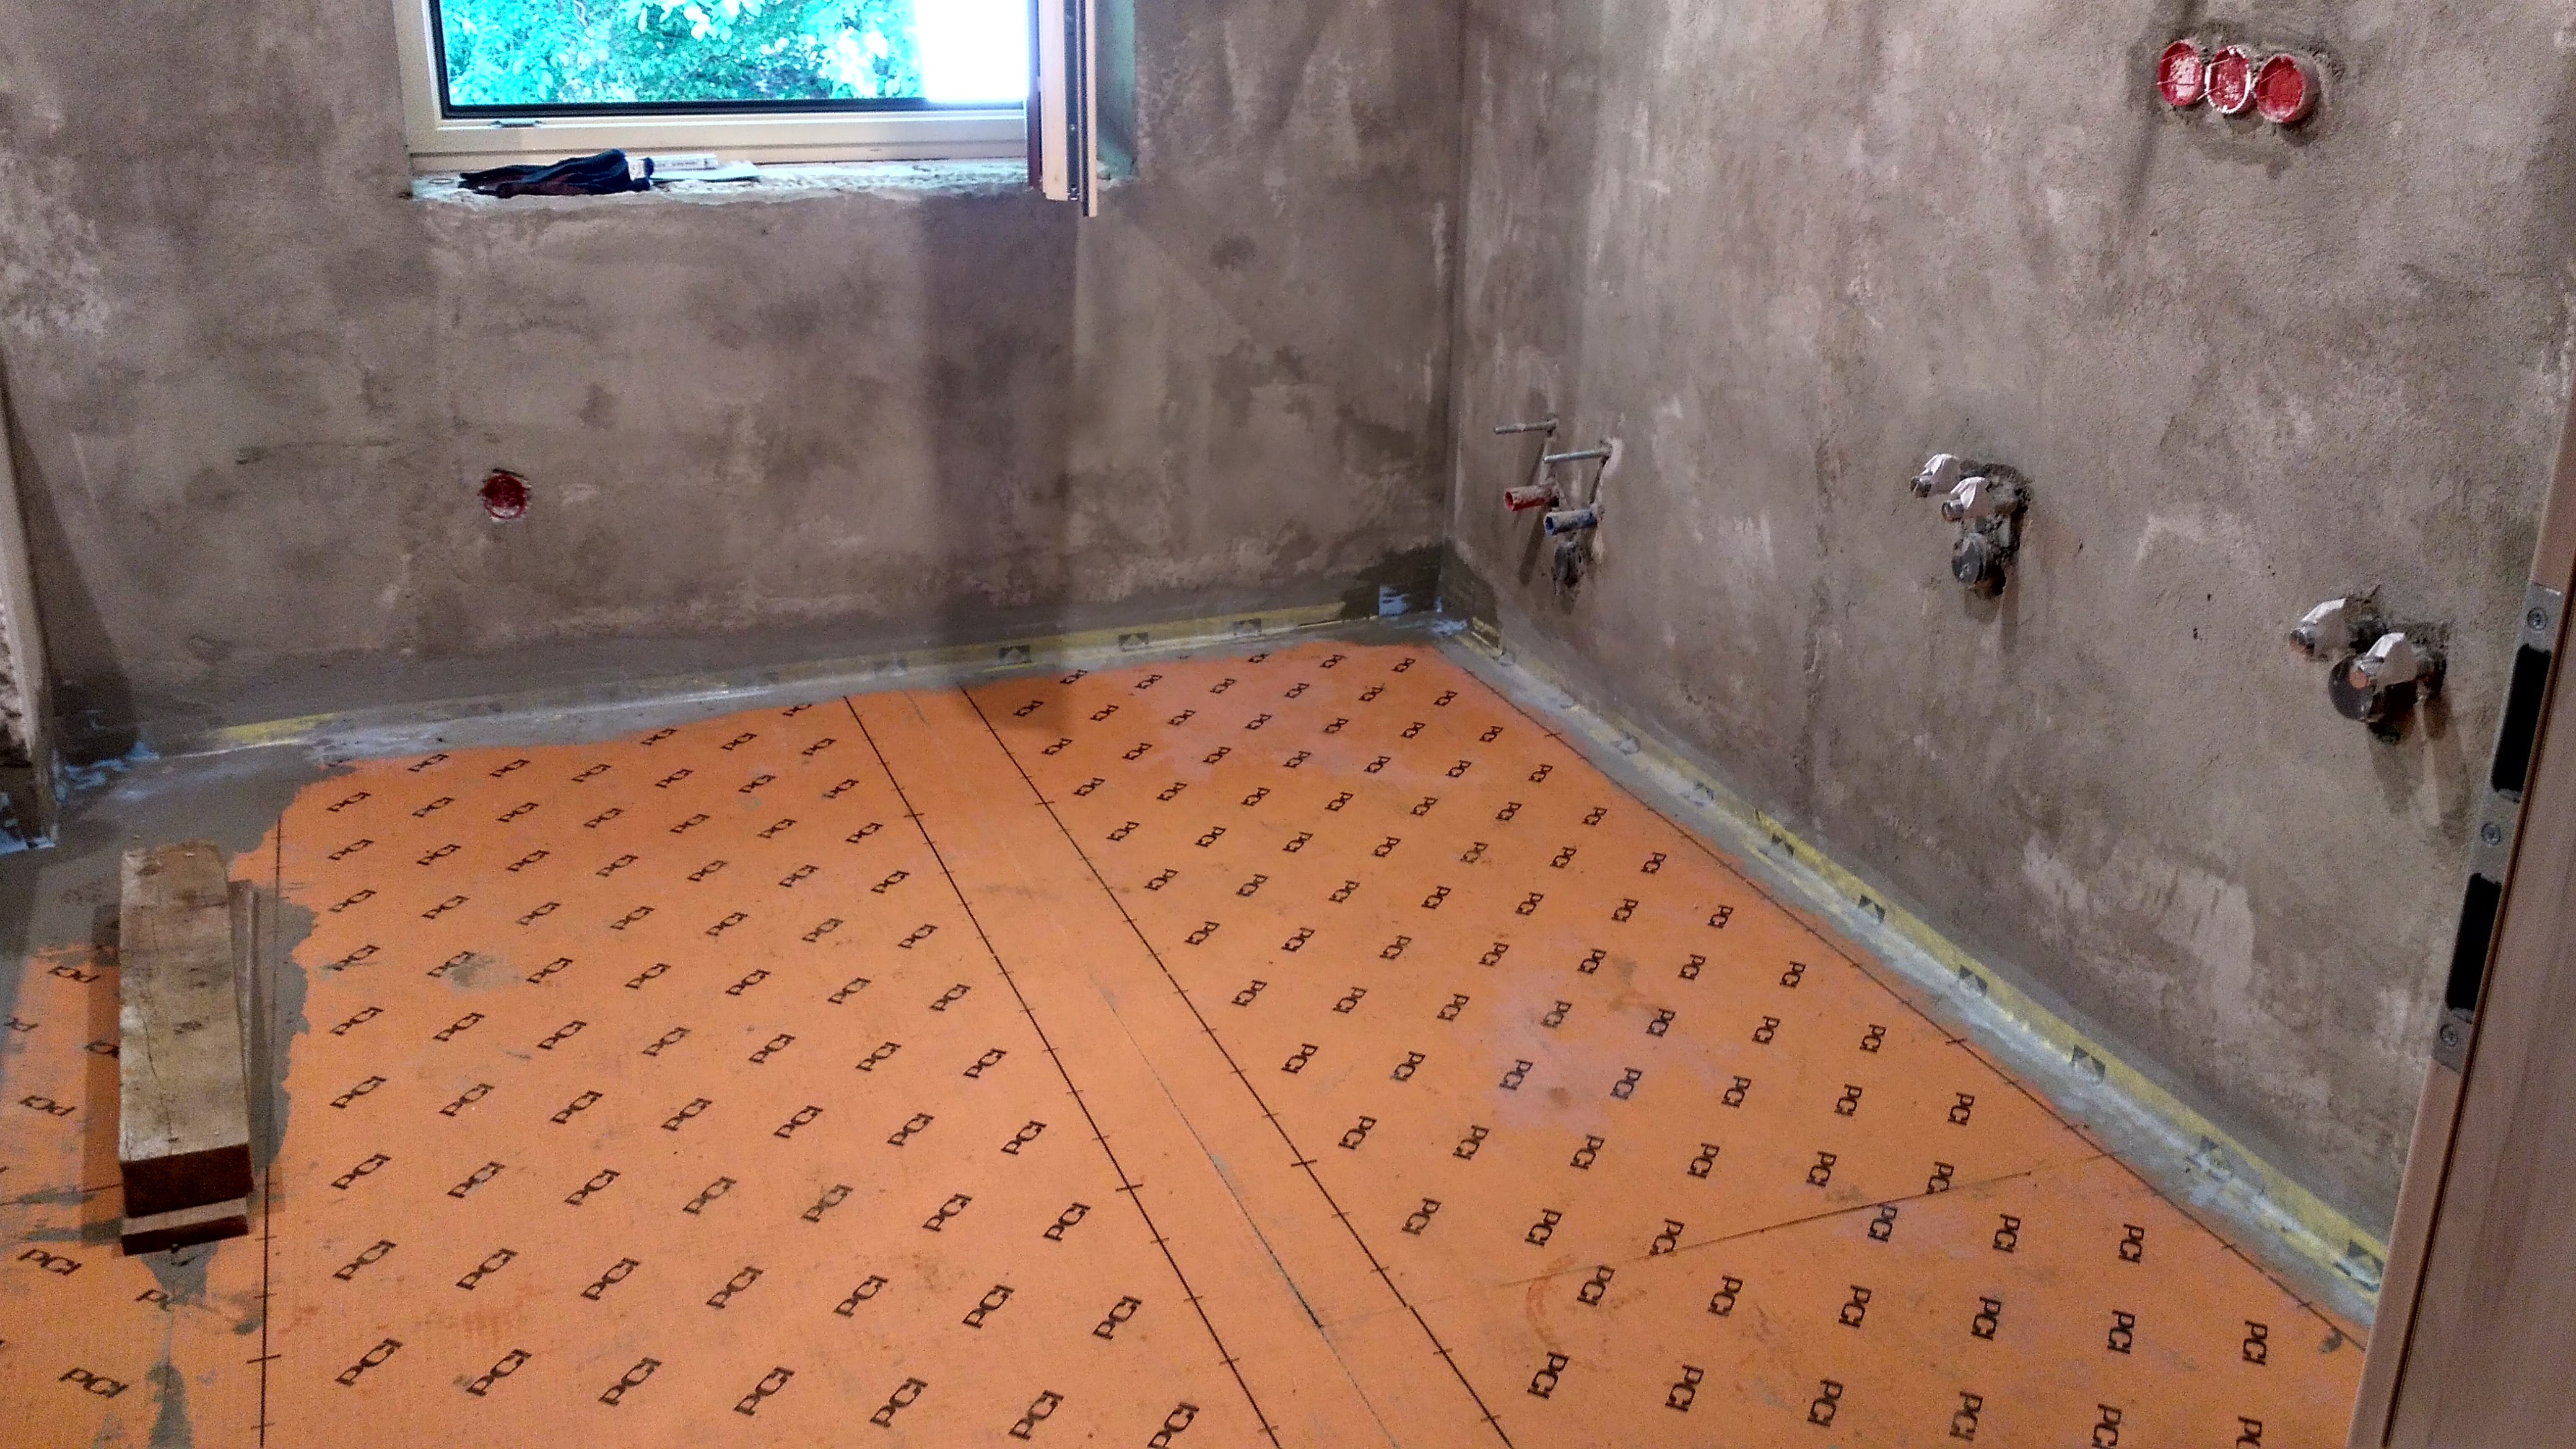
\includegraphics[scale=0.1]{Resources/Praktikum/IMG_20180801_114820_HDR.jpg}
		\label{bodenDicht}
		\caption{Boden mit Entkopplungsmatten und Abdichtbändern in den Ecken}	
	\end{center}
\end{figure}

\begin{figure}[h]
	\begin{center}
		\noindent\includegraphics[scale=0.1]{Resources/Praktikum/IMG_20180801_114836_HDR.jpg}
		\label{eckeDicht}
		\caption{Ecke mit Abdichtbändern}	
	\end{center}
\end{figure}

Nun mussten die Wände der Dusche den Vorschriften gemäß wasserdicht gemacht werden. Nur Fliesen alleine bieten einen ungenügenden Schutz gegen Wasser. Dazu strich ich die gesamte Dusche mit Lastogum, einer Flüssigfolie aus. Diese bildet auf der Mauer eine Wasserundurchlässige Schicht. In den Kanten der Dusche mussten Abdichtbänder eingeklebt werden. Dazu schnitt ich nach Augenmaß die Bänder zurecht. Anschließend strich ich dick Flüssigfolie in die Kanten und klebte das Abdichtband ein (siehe Abbildung \ref{duscheDicht}). Währenddessen bestrich der Fliesenleger den Periplanboden mit Hilfe einer feinzahnigen Kelle mit Kleber und legte die Entkopplungsmatten darauf (siehe Abbildung \ref{bodenDicht}). Die Kelle mit 2mm Stärke benutzte er, damit er den Kleber nicht zu dick aufträgt, damit die Matte nicht schwimmt und wellig wird. Daraufhin klebte ich die Abdichtbänder auch in die Kanten des Bodens, auf die Entkopplungsmatten. Der Fliesenleger klebte danach noch Abdichtecken in alle Ecken des Raums, um ihn komplett wasserdicht zu machen (siehe Abbildung \ref{eckeDicht}). Anschließend grundierten wir den Boden und alle Wände. Dann war alles bereit zum Fliesenverlegen.

\subsection{Fliesen verlegen und verfugen}

Der Fliesenleger wollte zuerst die Wandfliesen verlegen. Dazu bestimmte er anfangs noch einmal ganz genau die Länge der ersten Wand. Er bestimmte zusätzlich ob der Boden entlang der Wand gerade verlief, oder ob sich Unebenheiten zeigten. Damit wollte der den Verschnitt bestimmen, den er am Boden haben wird, oder ob der, bei geradem Boden, ganze Fliesen bis nach unten verlegen konnte. Er wollte ca. auf Schulterhöhe mit dem Verlegen beginnen. Dazu zeichneten wir eine horizontale Orientierungslinie mit einer Schlagschnur an. Durch diese Linie konnte er sichergehen, dass die Wandfliesen nicht schief wurden, wenn er von einer Seite der Wand zur anderen verlegte. Er strich mit einer gezahnten Kelle Kleber, genug für zwei aneinanderliegende Fliesen, an die Wand und klebte eine Fliese ein. Beim Einkleben der zweiten Fliese ließ er für die Fuge ca. 5mm Platz zur ersten Fliese. Das machte er nach Augenmaß, ohne Abstandshalter. So klebte er eine Linie Fliesen vom einen Ende der Wand zum Anderen, entlang der Orientierungslinie ein. Bis jetzt konnte er dafür ganze Fliesen verwenden, die letzte musste er zuschneiden.

\begin{figure}[h]
	\begin{center}
		\noindent\includegraphics[scale=0.1]{Resources/Praktikum/IMG_20180806_081044_HDR.jpg}
		\label{wandFlieseSchneiden}
		\caption{Geschnittene Fliesen am Ende der ersten Wand}	
	\end{center}
\end{figure}

\begin{figure}[h]
	\begin{center}
		\noindent\includegraphics[scale=0.1]{Resources/Praktikum/IMG_20180807_120442_HDR.jpg}
		\label{schneider}
		\caption{Schneidebrett}	
	\end{center}
\end{figure}

Er maß den Abstand der letzten Fliese zur Wand. Auf seinem Fliesenschneider konnte er das Maß darauf einstellen, legte die Fliese ein, fuhr einmal mit dem Schneider darüber und brach das unbenötigte Stück entlang der Schnittlinie ab. Der gesamte Vorgang dauerte nicht länger als eine Minute.

Die zugeschnittene Fliese brachte er am Ende der Wand an. Anschließend klebte er die zwei Reihen darunter usw. ein (siehe Abbildung \ref{wandFlieseSchneiden}). Danach schlugen wir wieder eine horizontale Orientierungslinie an die Wand. Das machten wir regelmäßig, um zu gewährleisten, dass die Fliesenreihe nicht schief wurde. So flieste er die gesamte Wand, während ich ihm die Fliesen reichte.

\begin{figure}[h]
	\begin{center}
		\noindent\includegraphics[scale=0.1]{Resources/Praktikum/IMG_20180806_081011_HDR.jpg}
		\label{ersteWand}
		\caption{Fertige erste Wand und Anfang der Zweiten}	
	\end{center}
\end{figure}

Sobald die erste Wand fertig verfliest war begann er mit den anderen und ich fing an die Fliesen zu verfugen. Dazu strich ich mit einer Kelle dick Fugenmasse in die Zwischenräume der Fliesen. Anschließend wischte ich mit einem feuchten Schwamm darüber, um die überschüssige Fugenmasse abzutragen und der Fuge ihr richtiges Aussehen zu geben. Zum Schuss zog ich den frisch ausgewaschenen Schwamm einmal komplett von oben nach unten über die Wand, um die Fliesen sauber zu waschen. So ging ich auch bei den anderen Wänden vor. [TODO: evtl Fenster Geschichte einfügen)

\begin{figure}[h]
	\begin{center}
		\noindent\includegraphics[scale=0.1]{Resources/Praktikum/IMG_20180807_112239_HDR.jpg}
		\label{orientierung}
		\caption{Orientierungslinie zum Verlegen der Bodenfliesen}	
	\end{center}
\end{figure}

Nach dem Verlegen der Wände begann er mit dem Boden. Durch den Periplanboden war sichergestellt, dass keine Unebenheiten vorhanden sind. Sollte die Mitte des Raumes beispielsweise einen Abfluss haben und man müsste den Boden zu diesem abfallen lassen, müsste der Fliesenleger das beim Verlegen mit einplanen. Hier hatten wir aber einen ebenen Boden. Nun zeichneten wir mit der Schlagschnur wieder eine Orientierungslinie parallel zur Wand ein, ca. so weit von dieser entfernt, wie die Breite zweier aneinandergelegter Fliesen (siehe Abbildung \ref{orientierung}). Ich platzierte einige Bodenfliesen so, dass der Fliesenleger direkt darauf zugreifen kann, während er am Boden kniet und die Fliesen verlegt. Er strich den Kleber auf den Boden und verteilte ihn mit einer gezahnten Kelle. Danach legte er die Fliesen darauf. Den Abstand zweier Fliesen für die Fuge bestimmte er per Augenmaß. Die Orientierungslinie diente dazu, dass die Fliesen nicht schief wurden, da er alles nach Augenmaß verlegte. 

Nachdem er zwei Reihen Fliesen verlegt hatte, stand er auf und wir zeichneten eine weitere Orientierungslinie, zwei Fliesenbreiten weiter, ein. Dann wiederholte sich der ganze Prozess, bis der Boden komplett verlegt war. Mir viel dabei auf, dass der Arbeitsfluss des Fliesenlegers durch das anzeichnen der Orientierungslinie immer wieder unterbrochen wurde. 

Zum Schluss, nachdem der Kleber eine Nacht ausgehärtet hatte, verfugte ich die Bodenfliesen noch. Dazu strich ich, wie beim Verfugen der Wandfliesen, Fugenmasse zwischen die Fliesen, wischte mit feuchten Schwamm darüber, bis sie das ge-wünschte Aussehen hatten und wusch die Fliesen anschließend mit dem Schwamm sauber. Nun war der gesamte Raum gefliest.

\subsection{Finale Schritte}

Nach dem Fliesen und Verfugen müssen noch ein paar kleine Schritte durchgeführt werden, um die Arbeit fertigzustellen. Wurden beispielsweise große, schwere Wand-fliesen verlegt, wurden Abstandshalter zwischen zwei Fliesen geklemmt, damit diese nicht zusammenrutschen und die Fuge so zerstören. Diese Abstandshalter müssen jetzt entfernt werden, und die Löcher in der Fuge geschlossen.

Die Fliesen wurden verlegt, bevor der Türstock eingebaut wurde. Nachdem dieser eingesetzt wurde, mussten die Zwischenräume zwischen Türstock und Fliesen verfugt werden. Dazu spritzte der Fliesenleger Acrylsilikon hinein und strich es mit einem Schaber glatt. Acrylsilikon hat die Eigenschaft, Farbe, mit welcher er überstrichen wird, aufzunehmen und so besser zu halten.

\subsection{Besorgungsfahrten}
Um den Lesefluss nicht zu unterbrechen, habe ich Besorgungsfahrten in den Baumarkt oder Fahrten in das Lager nicht aufgenommen. Hier möchte diese zwei Aspekte kurz beschreiben.

Der Fliesenleger hat ein privates Lager, in dem er nicht verbrauchte Materialien, seine Utensilien, wie Kellen und Eimer, und Werkzeuge, wie ein Multitool aufbewahrt. Den Lagerbestand hat er im Kopf. Am Anfang jedes Tages fuhren wir zuerst in das Lager und packten die nötigen Sachen ein. Da sein Auto nicht zu groß war, war die Tagesplanung wichtig, um unnötige Lagerfahrten während des Tages zu vermeiden.

Hatte er etwas nicht im Lager, was wir für die Baustelle brauchten, kauften wir es im Baumarkt ein. Alle Handwerker sind gut mit Baumärkten vernetzt. Sie können anrufen und vorbestellen. Die Baumärkte bereiten die Materialien dann vor, sodass man sie schnell abholen kann. Noch dazu speichern die Märkte die Daten des Handwerkers und können so direkt Abrechnungen erstellen und ihm zukommen lassen. Das spart wiederum Zeit, da man nicht zum Bezahlen in der Schlange stehen muss.

\section{Herausgearbeitete Ansatzpunkte}

Durch die Ethnographie zeigt sich, dass die meisten Arbeitsschritte eines Fliesenlegers relativ schnell auch präzise ausgeführt werden können. Kleber und sonstige Stoffe anzumischen erfordert keine Hilfe. Wände mit Flüssigkleber, Boden oder Wände mit Fliesenkleber und Fugen mit Fugenmasse zu bestreichen, lässt sich mit geeignetem Werkzeug präzise und schnell ausführen. Auch für das Schneiden und Einkleben der Fliesen sind die Maße schnell genommen und eingezeichnet. Der Fliesenleger hat eine einstudierte Routine und arbeitet dadurch zügig.
Allerdings werden zwei Ansatzpunkte deutlich, bei denen der Handwerker Unterstützung benötigt. Das sind die Planung mit dem Kunden im Kundengespräch, wobei Kunde und Fliesenleger gerne aneinander Vorbeireden, oder der Kunde sich das Ergebnis nicht vorstellen kann, sowie das Fliesenlegen, wo der Fliesenleger durch das anschlagen der Orientierungslinie aus dem Arbeitsfluss gerissen wird.

\subsection{Unterstützung beim Fliesenlegen}

Wenn der Fliesenleger ohne Orientierungslinie arbeitet, läuft er Gefahr, den Boden irgendwann schief zu verlegen. Ohne sie kann er also nicht arbeiten. Jedes mal wenn er diese mit der Schlagschnur anzeichnet, muss er aufstehen, die Endpunkte der Linie markieren und diese einzeichnen. Das wird nochmal schwerer, wenn er allein arbeitet, da man eine Schlagschnur mit zwei Personen leichter benutzen kann. Das anzeichnen reißt ihn zusätzlich aus seinem Arbeitsfluss. Könnte der Fliesenleger den Schritt des Anzeichnens einer Orientierungslinie umgehen, könnte er ungehindert weiterarbeiten, sofern er einen Helfer hat der ihm die Fliesen reicht und Kleber für ihn anrührt. Dadurch kann er viel Zeit sparen und es wäre gleichzeitig auch bequemer für ihn.

\subsection{Unterstützung beim Kundengespräch}

Das Kundengespräch war chaotisch und sehr unstrukturiert. Die Vorstellungskraft der Kunden, vor allem wenn diese Laien sind, ist sehr begrenzt. Dadurch ist es schwer mit ihnen über Änderungen zu diskutieren. Der Fliesenleger hat das Bild, durch seine Erfahrung besser im Kopf. Jedoch ist es schwer das in Worte zu fassen die der Kunde versteht. Es wäre deutlich einfacher über Ideen zu sprechen, wenn man diese direkt vor sich sehen würde.

Das Ergebnis vorab schon zu sehen hat noch weiter Vorteile:

\begin{itemize}
	\item Der Kunde kann während dem Planungsprozess bereits gezielt Feedback geben. Ansonsten kann er das erst spät im Prozess, wodurch es erheblich schwerer ist darauf einzugehen.
	\item Dadurch kann der Vertrag mit dem Kunden, was der Fliesenleger zu tun hat, genauer ausgearbeitet werden.
	\item Die Zusammenarbeit mit anderen Handwerkern ist einfacher koordinierbar.
	\item Das geplante Muster dient als visuelle Vorlage für den Fliesenleger. Dadurch muss er das Bild nicht nur im Kopf haben.
	\item Bereits beim Planen des Raumes lässt sich der Verschnitt gut abschätzen.
\end{itemize}

Die Unterstützung bei der Orientierungslinie würde dem Fliesenleger Zeit ersparen und ein Visualisierungstool würde ihm die Planung erleichtern. Daran kann man ansetzen, um technische Unterstützungssysteme zu implementieren.
\chapter{Design des Artefakts}

In diesem Kapitel wird die Entwicklung der HoloLens Planner App zur Unterstützung von Fliesenlegers, welche für die Microsoft HoloLens entwickelt wird, beschrieben. Zum Entwickeln wurde Unity verwendet. Das Hololens Toolkit stellte benötigte Funktionalitäten zur Verfügung, welche beim Entwickeln für die Microsoft HoloLens essentiell sind.
Es wird nach der Methode für gestaltungsorientierte Forschung von Peffers (siehe Sektion \ref{sec:gestForsch}) vorgegangen. Die Probleme von Handwerkern, genauer Fliesenlegern, werden herausgearbeitet. Daraus werden Ziele für die zu entwickelnde Applikation abgeleitet. Diese Anwendung wird anschließend in einem iterativen Prozess über fünf Phasen entwickelt. Abschließend werden die Ergebnisse kommuniziert.

\section{Problemidentifikation und Motivation}

Aus der Ethnographie geht hervor, dass beim Verlegen der Fliesen Zeit verloren geht. Der Handwerker muss dabei jedes mal seinen Arbeitsfluss unterbrechen und im Raum nachmessen, um die Orientierungslinie korrekt anzuzeichnen. Dies macht er mit einer Schlagschnur, was jedoch schwierig wird, wenn er allein arbeitet. Müsste es diese Linie nicht anzeichnen, könnte er, unterstützt durch einen weiteren Arbeiter, der ihm Fliesen reicht, den gesamten Boden am Stück verlegen. Diese Linie ist jedoch essentiell wichtig, damit die Fliesen beim Verlegen nicht schief werden.

Laut Fokusgruppe und Ethnographie wäre ein Werkzeug, um den Raum zu erfassen und so die Planung zu vereinfachen, hilfreich. Die Wandlängen, Winkel und Unebenheiten zu messen nimmt einiges an Zeit in Anspruch. Schreibt der Handwerker sich dies nicht auf, hat er die Maße nur für den nächsten Arbeitsschritt im Kopf und muss das Vermessen oft wiederholen. Das kostet den Handwerker viel Zeit, wie in der Fokusgruppe hervorgehoben. Fliesenleger müssen bei diesem Schritt auch an den Fliesenverschnitt denken. Sie wollen Fliesen, die auf weniger als 2cm zurechgeschnitten werden müssen unbedingt vermeiden. Eine visuelle Darstellung des Raumes wäre dabei förderlich. 

Ein weiteres Problem ist die Abstimmung mit anderen Handwerkern. Erledigte oder geplante Aufgaben werden oft per Telefon kommuniziert, wodurch viel Misskommunikation und Fehler entstehen können. Besonders in dem Fall, dass ein Handwerker das Kundengespräch leitet und seine Kollegen anschließend über die Pläne informiert, wie aus der Fokusgruppe hervorgeht. Der Handwerker aus der Ethnographie merkte an, dass der Vertrag mit dem Kunden aus selbem Grund häufig nicht richtig spezifiziert ist und er so falsch umgesetzt wird.

Das größte Problem, bei welchem sich die Handwerker der Fokusgruppe, sowie der Ethnographie einig waren, ist die mangelnde Vorstellungskraft der Kunden. Der Handwerker kann sich das Ergebnis seiner Arbeit im Rohbau bereits vorstellen, da er die Erfahrung hat, der Kunde jedoch nicht und mit Worten ist so etwas schwer zu beschreiben, wie in der Ethnographie erläutert wird. Dadurch ist es für den Handwerker auch schwer dem Kunden zu zeigen, warum er etwas anders machen würde als dieser sich vorstellt. Oft reden Handwerker und Kunde bei diesen Gesprächen aneinander vorbei. Einen technischen Bauplan versteht der Laie auch nicht und Skizzen helfen nur mäßig. Dabei kommt es oft zu Ambiguität in den Kundengesprächen.

\section{Ziele der Lösung}

Mit der Lösung wird angestrebt, die Pläne des Fliesenlegers zu visualisieren und ihn bei der Arbeit zu unterstützen. \\
Lassen sich die Pläne des Handwerkers direkt betrachten, ist es einfacher für beide Parteien Änderungen vorzuschlagen, zu positionieren und zu beschreiben. Am besten sollte dies direkt im Rohbau möglich sein. Durch die Visualisierung können Pläne auch zwischen Handwerkern deutlicher kommuniziert werden. \\
Zur Unterstützung beim Fliesenlegen soll das erstellte Programm den Raum vermessen können und dies auch automatisch dokumentieren, sodass die Informationen jederzeit eingesehen werden können. Außerdem soll es möglich sein zu vermeiden, dass die Fliesen beim verlegen schief werden. Es wird also eine virtuelle Orientierungslinie oder Ähnliches benötigt.

\section{Entwicklung des Artefakts}

Die folgenden Abschnitte beschreiben die einzelnen Schritte der Entwicklung der App. Mit kleinen Evaluationsrunden wurde diese über fünf Iterationen verbessert und benutzerfreundlicher gemacht.

\subsection{Phase 1}

\subsubsection{Gestaltung und Entwicklung}

Anfangs wurde der Fokus auf die Funktionalität zum Boden bestimmen und Fliesen verlegen gelegt. Unterstützung bei der Arbeit des Fliesenlegers wird ab Phase 4 hinzugefügt. 

Zur Navigation durch die Funktionen der Applikation wird ein Menü designed mit den Schaltflächen \enquote{Bodenfläche abstecken}, sowie \enquote{Fliesen verlegen}. Das dient dazu, navigieren zu können, falls die Bodenfläche angepasster werden soll.

\begin{figure}[h]
	\begin{center}
		\noindent\includegraphics[scale=0.7]{Resources/Artefakt/bodenAbstecken.png}
		\label{abstecken}
		\caption{Abstecken des Bodens}	
	\end{center}
\end{figure}

Die Microsoft HoloLens besitzt \textbf{spatial mapping}, was sie dazu nutzt, um sich ein internes Bild ihrer Umgebung zu erzeugen. Diese Funktion unterscheidet allerdings nicht zwischen \enquote{Wand}, \enquote{Boden} oder \enquote{Decke}. Daher muss der Boden händisch festgelegt werden. Dazu platziert der Nutzer in den Ecken des Raumes kleine Punkte, welche automatisch durch Linien miteinander verbunden werden (siehe Abbildung \ref{abstecken}). Durch \enquote{Klicken \& Halten} wird daraus die Bodenfläche erstellt, auf der anschließend die Fliesen verlegt werden sollen.

\begin{figure}[h]
	\begin{center}
		\noindent\includegraphics[scale=0.50]{Resources/Artefakt/auswahlAlt.png}
		\label{fliesenwahlAlt}
		\caption{Altes Menü zur Fliesenauswahl}	
	\end{center}
\end{figure}

\begin{figure}[h]
	\begin{center}
		\noindent\includegraphics[scale=0.55]{Resources/Artefakt/detailAlt.png}
		\label{fliesendetailAlt}
		\caption{Altes Menü für Detailansicht}	
	\end{center}
\end{figure}

Das Fliesenmenü präsentiert in einem 3x2 Grid eine Auswahl an verschiedenen Fliesen (siehe Abbildung \ref{fliesenwahlAlt}). Wählt der Nutzer eine davon, öffnet sich eine Detailansicht der Fliese, welche alle Informationen dazu in Textfeldern anzeigt (siehe Abbildung \ref{fliesendetailAlt}). Diese beinhalten Breite, Länge, Fugenweite und die Textur der Fliese. In dieser Ansicht ist es auch möglich die Fliese zu bearbeiten. Zusätzlich können neue Fliesen angelegt und in den Katalog eingefügt werden.

\begin{figure}[h]
	\begin{center}
		\noindent\includegraphics[scale=0.4]{Resources/Artefakt/bodenVerlegt.png}
		\label{bodenVerl}
		\caption{Virtuell verlegte Fliesen}	
	\end{center}
\end{figure}

Wurde die Bearbeitung abgeschlossen, müssen die Fliesen verlegt werden. Dabei erschien es am besten für einen Prototypen, die Fliesen entlang einer Kannte des Bodens zu verlegen. Dafür wählt der Nutzer einen Eckpunkt der Fläche als Startpunkt und einen weiteren als Richtungspunkt. Sind diese gewählt, verlegt die Applikation die Fliesen virtuell (siehe Abbildung \ref{bodenVerl}).

\subsubsection{Demonstration des Artefakts}

Zur Demonstration des ersten Prototypen wurden zwei Studenten der Fakultät Informatik der Technischen Universität München gewählt. Sie sollten die Applikation in einem teilweise möblierten Raum testen. Vor dem Test wurde nur festgelegt, was das Ergebnis sein sollte. Währenddessen wurde versucht keine Anweisungen gegeben.

\subsubsection{Evaluation}

Das Szenario war für die Studenten, obwohl sie technisch aversiert sind, schwer ohne Anweisungen durchführbar. Es vielen dabei einige Verbesserungsmöglichkeiten auf. 

Beim Abstecken der Bodenfläche hat der Nutzer keine Möglichkeit Fehler zu beheben. Wurde ein Punkt, evtl. durch einen unbeabsichtigten Klick, falsch positioniert, gab es keine Option, um das rückgängig zu machen. \\
Die Daten in den Textfeldern waren sehr klein geschrieben und daher schwer zu lesen. Noch dazu bemängelten die Probanden, dass es nicht elegant wirke. \\
Aus der Detailansicht zum Bearbeiten der Fliesen konnte man nicht auf die Fliesenauswahl zurücknavigieren, was die Probanden auch bemängelten.

\subsection{Phase 2}

\subsubsection{Gestaltung und Entwicklung}

Um Fehler beim Abstecken der Bodenfläche beheben zu können, wurde eine Funktion eingebaut, mit der der zuletzt gesetzte Punkt durch Anklicken gelöscht werden kann. 

\begin{figure}[h]
	\begin{center}
		\noindent\includegraphics[scale=0.4]{Resources/Artefakt/auswahl.png}
		\label{auswahl}
		\caption{Neues Design der Fliesenauswahl}	
	\end{center}
\end{figure}

Das Design der Fliesen Detailansicht wurde umgebaut, um es mit natürlichen, selbsterklärenden Schaltflächen intuitiver zu machen und um Textboxen zu eliminieren. Dabei wurde auch das gesamte Design der App dunkler gemacht (siehe Abbildung \ref{auswahl}). Zusätzlich wurde eine Einstellungsmöglichkeit für die Tiefe der Fliesen eingefügt (siehe Abbildung \ref{detail}).

\begin{figure}[h]
	\begin{center}
		\noindent\includegraphics[scale=0.4]{Resources/Artefakt/detail.png}
		\label{detail}
		\caption{Neues Design der Detailansicht}	
	\end{center}
\end{figure}

Für den Wechsel zwischen Fliesenauswahl Ansicht und Fliesen Detailansicht wurde ein entsprechender Button eingefügt.

\subsubsection{Demonstration des Artefakts}

Es wurden erneut zwei Studenten der Fakultät für Informatik der TU München ausgewählt, um die Applikation zu testen. Dafür wurde der selbe teilweise möblierte Raum genutzt. Es wurde geplant während des Tests nur Anweisungen zu geben, wenn der Proband nicht weiter kommt.

\subsubsection{Evaluation}

Beide Probanden fanden das Erzeugen der Bodenfläche durch \enquote{Klicken \& Halten} wenig intuitiv. Außerdem viel auf, wenn man eine neue Bodenfläche erstellen möchte, bleibt die alte weiter bestehen. Das sollte nicht passieren. \\
In der neuen Detailansicht war nicht ersichtlich welcher Button zum Verlegen der Fliesen führt, da dafür nun Symbole, statt Worte als Beschreibung verwendet wurden. \\
Auch das Verlegen der Fliesen wurde von einem Probanden als nicht intuitiv beschrieben.

\subsection{Phase 3}

\subsubsection{Gestaltung und Entwicklung}

Es wurde Tutorialtext eingefügt, welcher das Abstecken des Bodens beschreibt. Dieser geht auch darauf ein, dass man zum erstellen \enquote{Klicken \& Halten} muss (siehe Abbildung \ref{tutBoden}). \\
Das Verlegen der Fliesen wird jetzt auch mit Tutorialtext beschreiben (siehe Abbildung \ref{tutFliesen}). \\
Diese Tutorialtexte sind nicht irgendwo im Blickfeld fixiert, sondern folgen dem Gaze. Damit der Text nicht beim Arbeiten am Boden stört, wurde die Option eingefügt, ihn im Raum zu fixieren. Ein weißer Pfeil deutet dann auf diesen, damit man ihn wiederfindet. Die Information die UI so zu erstellen, stammt auf diesem Video: \url{https://www.youtube.com/watch?v=sX6yKHmN1qM}.

\begin{figure}[h]
	\begin{center}
		\noindent\includegraphics[scale=0.4]{Resources/Artefakt/bodenText.png}
		\label{tutBoden}
		\caption{Tutorialtext zum Abstecken des Bodens}	
	\end{center}
\end{figure}

\begin{figure}[h]
	\begin{center}
		\noindent\includegraphics[scale=0.4]{Resources/Artefakt/verlegenText.png}
		\label{tutFliesen}
		\caption{Tutorialtext zum Verlegen der Fliesen}	
	\end{center}
\end{figure}

Falls bereits ein Boden erstellt wurde, dieser jedoch nicht genau genug ist und der Nutzer daher einen neuen erstellt, wird der alte Boden automatisch gelöscht.

Damit die Funktionalität der Symbole der Buttons im Fliesen Detailmenü ersichtlicher ist, wurde ein Beschreibungstext eingefügt, welcher erscheint, wenn der Nutzer den Gaze darauf richtet.

\subsubsection{Demonstration des Artefakts}

Dieses mal wurde die Applikation erneut mit zwei Studenten der TU München, als auch mit einem Wissenschaftlichen Mitarbeiter. Dafür wurde der selbe Raum wie bei den ersten Tests verwendet. Anweisungen wurden nur wenn nötig gegeben.

\subsubsection{Evaluation}

Beim Abstecken des Bodens können teilweise Punkte nicht gesetzt werden. Das behindert die Funktionalität und frustriert den Nutzer. Der wissenschaftliche Mitarbeiter merkte an, dass es für die Genauigkeit der Bodenfläche gut wäre, wenn man die Eckpunkte nachträglich verschieben und so präziser in den Ecken positionieren könnte. \\
Das Menü folgt dem Gaze un behindert so teilweise das Verlegen der Fliesen.

\subsection{Phase 4}

\subsubsection{Gestaltung und Entwicklung}

Die Eckpunkte sind nur auf \enquote{gemappetem} Areal setzbar, also Boden, den die HoloLens schon selbst gescanned und realisiert hat. Um das zu verdeutlichen wird das spatial mapping nun mit einem grünen Gitter angezeigt (siehe Abbildung \ref{abstecken}). So erkennt der Nutzer genau, welche Teile des Raums bereits gemapped sind und welche noch nicht.

\begin{figure}[h]
	\begin{center}
		\noindent\includegraphics[scale=0.5]{Resources/Artefakt/punktVersch.png}
		\label{pfeile}
		\caption{Pfeile zum Verschieben der Eckpunkte}	
	\end{center}
\end{figure}

\begin{figure}[h]
	\begin{center}
		\noindent\includegraphics[scale=0.4]{Resources/Artefakt/bodenUpDown.png}
		\label{pfeileBoden}
		\caption{Pfeile zum verschieben der Bodenfläche}	
	\end{center}
\end{figure}

Sobald die Bodenfläche erstellt ist, kann der Nutzer die einzelnen Eckpunkte nun verschieben. Wählt er einen davon aus erscheinen rundherum Pfeile (siehe Abbildung \ref{pfeile}). Mit diesen kann er den Punkt in 0,5cm Schritten in beliebige Richtungen bewegen und die Eckpunkte so präziser setzen. Zusätzlich wurde vorbeugend die Funktionalität eingebaut, mit Pfeilen die gesamte Fläche hoch oder runter zu bewegen (siehe Abbildung \ref{pfeileBoden}). Das soll helfen, falls Teile der Bodenfläche im \enquote{realen Boden verschwinden}.

Damit das Menü beim Arbeiten nicht mehr stört, wurde eine \textit{pin-Funktion} implementiert. Mit Klick auf die Schaltfläche wird das Menü an eine Stelle im Raum gepinnt und kann so auch wieder gelöst werden (siehe Abbildung \ref{menue}). Ein weißer Pfeil leitet den Nutzer zum Menü zurück, falls er es verlieren sollte.

\begin{figure}[h]
	\begin{center}
		\noindent\includegraphics[scale=0.4]{Resources/Artefakt/verlegeassistent.png}
		\label{assistent}
		\caption{Assistent zum Fliesenverlegen}	
	\end{center}
\end{figure}

\begin{figure}[h]
	\begin{center}
		\noindent\includegraphics[scale=0.4]{Resources/Artefakt/menue.png}
		\label{menue}
		\caption{Startmenü mit Pin-Button oben rechts}	
	\end{center}
\end{figure}

In dieser Iteration wurde auch ein Assistent zum Fliesenverlegen implementiert. Durch einen neuen Button im Menü kann dieser aktiviert werden. Das ist allerdings erst nach dem Verlegen der Fliesen möglich. Er lässt die Fliesen verschwinden und zeigt nur noch deren Fugen in blau an (siehe Abbildung \ref{assistent}). So stellt er dem Handwerker ein Gitter, in welches er nur noch die echten Fliesen einzulegen braucht.

\subsubsection{Demonstration des Artefakts}

Diese Demonstration wurde mit zwei Wissenschaftlichen Mitarbeitern der Fakultät für Wirtschaftsinformatik der TU München durchgeführt. Sie fand im selben Raum statt. Diesmal wurde den Probanden ein Szenario vorgegeben. Sie sollten eine festgelegte Fläche abstecken, darauf Fliesen verlegen und alle Funktionen des HoloLens Planners einmal testen.

\subsubsection{Evaluation}

Die Tutorialtexte und alle anderen waren bis jetzt auf Englisch. Da die App zum Abschluss noch mit deutschen Handwerkern getestet werden sollte, wäre es von Vorteil diese auf Deutsch zu übersetzen. \\
Die Pfeile zum Verschieben der Punkte wurden, laut der Probanden, zu groß angezeigt. Dadurch verliert man beim Bedienen den Überblick.

\subsection{Phase 5}

\subsubsection{Gestaltung und Entwicklung}

Die Pfeile für das Verschieben der Punkte wurden verkleinert. Alle Texte der Applikation wurden ins Deutsche übersetzt.

\begin{figure}[h]
	\begin{center}
		\noindent\includegraphics[scale=0.4]{Resources/Artefakt/datenBoden.png}
		\label{daten}
		\caption{Daten zum verlegten Boden}	
	\end{center}
\end{figure}

Zu guter Letzt wurde die Funktionalität zum Anzeigen wichtiger Metriken umgesetzt. Im Bodenmenü kann der Fliesenleger nun einsehen, wie groß die Fläche in Quadratmetern ist und wie viel Umfang sie hat (siehe Abbildung \ref{daten}). Zusätzlich, vorausgesetzt der Handwerker hat virtuell bereits die Fliesen verlegt, zeigt diese Ansicht ihm die Anzahl der benötigten Fliesen an.

\subsubsection{Demonstration des Artefakts und Evaluation}

Die Finale Demonstration und Evaluation der HoloLens Planner Applikation mit allen Funktionalitäten wird mit Handwerkern durchgeführt. Die Durchführung und Ergebnisse davon werden im nächsten Kapitel kommuniziert. 
\chapter{Evaluation}

Dieses Kapitel beschreibt die finale Evaluation der HoloLens Planner App mit Handwerkern. Zu erst wird die Durchführung erklärt und anschließend die gewonnenen Erkenntnisse aus Fragebogen und den nachfolgenden Gesprächen. Dabei wird genauer darauf eingegangen, wie gebrauchstauglich die Applikation den Handwerkern erscheint, wie sie die Belastung bei ihrer Benutzung einschätzen, ob sie die Technologie Augmented Reality zur Unterstützung ihrer Arbeit in Zukunft akzeptieren würden, wie sie die Erfahrung mit der Applikation fanden und wie man diese noch entwickeln könnte. Es wurden sieben verwertbare Fragebögen und zehn Interviews erzeugt.

\section{Durchführung der Evaluation}

Die Tests wurden bei zehn Handwerkern einzeln, an unterschiedlichen Tagen, zu Hause mit der Microsoft HoloLens und der HoloLens Planner Applikation durchgeführt. Zur Ausführung der Tests wurde den Handwerkern anfangs grob der Umfang dieser Masterarbeit erklärt und was damit bezweckt wird. Anfangs wurde durch Literaturrecherche der aktuelle Stand der Digitalisierung in Handwerksbetrieben und KMUs festgestellt. Um die Materie der Arbeit auf dem Bau kennenzulernen und im Beruf eines Handwerkers Erfahrungen zu machen, die vorher nicht bestanden, wurde eine Ethnographie zum Handwerk des Fliesenlegers durchgeführt. Dadurch wurden Ansatzpunkte für die Unterstützung durch Technologie, genauer durch die Nutzung von Augmented Reality, für Fliesenleger gefunden. Aus diesen Funden wurde eine AR Applikation für die Microsoft HoloLens entwickelt, welche Handwerker beim Kundengespräch, durch virtuelles Fliesenverlegen, sowie beim Fliesen verlegen, durch einblenden eines blauen Rasters helfen soll. Diese Applikation gilt es nun mit Handwerkern zu testen und ihre Meinung darüber zu erheben. 

Die Daten wurden in 3 Phasen erhoben. 

\begin{itemize}
	\item Testen der Applikation in einem vordefinierten Szenario
	\item Ausfüllen des Fragebogens
	\item Unstrukturiertes Gespräch
\end{itemize}

Zum Testen wurde jeweils eine große, freie Fläche benötigt. Den Probanden wurde das Szenario erst erklärt und anschließend wurden sie durch die Applikation geleitet. Es ging darum einen viereckigen Boden im Raum zu markieren und Fliesen darauf zu verlegen, den Verlegeassistenten zu aktivieren und Daten über die Fläche auszulesen. Erst platzierte jeder Proband vier Eckpunkte im Raum. Diese mussten nicht zwingend in tatsächlichen Ecken platziert werden, da das teilweise aus Platzgründen auch nicht möglich war. Nachdem die Fläche so markiert wurde, wählte sie eine Fliese aus, die sie verlegen wollten. Breite und Länge dieser konnten sie beliebig modifizieren. Anschließend legten sie sie auf dem abgesteckten Boden aus. Es wurde ihnen Zeit gegeben sich im Raum zu bewegen und das Bild aufzunehmen. Anschließend aktivierten sie den Verlegeassistenten, welcher nur die Fugen in blau auf dem Boden anzeigt. Wieder hatten sie Zeit, um sich mit dem Feature auseinander zu setzen. Zuletzt öffneten sie erneut das Bodenmenü und bekamen die Daten Fläche, Umfang und Anzahl der Fliesen angezeigt. Damit war der Test beendet.

Von da ging es direkt, ohne viel Kommunikation zum Fragebogen über, den sie freiwillig ausfüllen sollten. Dabei wurde ihnen nur kurz erklärt, wie dieser auszufüllen war. Unterstützt wurden sie dabei nur, wenn ihnen ein Wort undeutlich war. Ansonsten wurde dabei nicht geredet und sie füllten den Fragebogen selbstständig aus.

Zum Abschluss wurde ein unstrukturiertes Gespräch mit jedem Probanden geführt. Dabei sollten diese einfach über ihre Gedanken zu dem Experiment sprechen. Falls das Gespräch stagnierte wurde es mit Fragen, wie zum Beispiel \enquote{Was fanden Sie gut an der Applikation}, \enquote{Welche Funktionalitäten würden Sie sich noch wünschen} oder \enquote{Was hat Ihnen an der Applikation nicht gefallen} wieder angekurbelt. Generell waren die Handwerker jedoch gut im Redefluss und brachten viele eigene Ideen ein und dachten die bisherige Idee weiter. Diese Gespräche wurden, nach Absprache mit den Probanden, teilweise aufgezeichnet. Während jeder Unterhaltung wurden Notizen angefertigt, welche die Aussagen der Handwerker indirekt festhielten.

\section{Diskussion der Ergebnisse}

Diese Sektion zeigt die Ergebnisse der, durch die Handwerker, ausgefüllten Fragebögen. Alle Daten die hier aufgezeigt werden beziehen sich auf die sieben verwertbaren Fragebögen, die korrekt ausgefüllt wurden. 

\begin{figure}[h]
	\begin{center}
		\includegraphics[scale=0.5]{Resources/Evaluation/allgemein.png}
		\label{allgemein}
		\caption{Erhobene allgemeine Daten}	
	\end{center}
\end{figure}

\begin{figure}[h]
	\begin{center}
		\includegraphics[scale=0.5]{Resources/Evaluation/playful.png}
		\label{playful}
		\caption{Erhobene Daten zur Playfulness}	
	\end{center}
\end{figure}

Alle Probanden waren männlich und zwischen 21 - 54 Jahre, fünf davon unter 40 Jahre und zwei über 40 Jahre, alt. Durchschnittlich gaben sie an mit der Technologie Augmented Reality gut vertraut zu sein. Das könnte auf die weite Verbreitung von VR in den letzten Jahren zurückzuführen sein und darauf, dass man diese Technologien häufig auf Messen oder sogar in Museen ausprobieren kann. Allerdings reichen die Angaben von nicht bis sehr vertraut. Im privaten Umfeld nutzen die Handwerker häufig technologische Hilfsmittel, im beruflichen hingegen eher weniger häufig (siehe Abbildung \ref{allgemein}). Das könnte ein weiteres Indiz sein, dass die Digitalisierung im Handwerk noch nicht weit fortgeschritten ist.

pl1 gibt an, dass die Nutzung von HoloLens Planner die Neugier aller Probanden stark anregt (siehe Abbildung \ref{playful}). Dieser Wert kann jedoch auf die Applikation selbst, als auch auf die Nutzung von AR generell bezogen sein. Augmented Reality stellt für die Handwerker zwar eine bekannte Technologie dar (siehe Abbildung \ref{allgemein}), jedoch wurde nicht erfragt, wie viele von ihnen schon eine VR oder AR Brille ausprobiert hatten. Die Probanden gaben an, dass sie nur mäßig die Zeit vergessen, während sie mit der Applikation arbeiteten. Nur ein Proband gab den höchsten Wert an, was sich mit seiner Aussage, er tauche komplett in die Erfahrung mit der Datenbrille ein abgleicht. Die teilweise Zustimmung, dass sie Freude am Arbeiten mit dem HoloLens Planner haben, lässt auf einen hohen Akzeptanzwert schließen.

Privat nutzt jeder Handwerker mindestens Computer und Smartphone. Über die Hälfte der Probanden gaben an auch von Tablets und teilweise Smartwatches Gebrauch zu machen. Das kann darauf hindeuten, dass sie technisch versiert sind und erklärt auch, warum sie die Nutzung der Microsoft HoloLens schnell, nach einmaligem Erklären, verstanden und umsetzen konnten. \\
Beruflich nutzen über die Hälfte der Handwerker Computer und Smartphone. Einzelne Probanden gaben an nur den Computer oder nur eine Smartphone zu nutzen. Knapp die Hälfte der Probanden setzen auch Tablets in ihrem Beruf ein und einer davon auch eine Smartwatch. Interessant ist, dass zwei der Handwerker Laser zum vermessen nutzen. Laut ihren Aussagen ermöglichen diese ihnen die Messungen noch genauer vorzunehmen, Messfehlern vorzubeugen und so auch besonders kleine Fugen von unter 3mm präzise und konsistent legen zu können. Das nur zwei der sieben Handwerker Laser verwenden kann darauf hindeuten, dass noch kein Großteil der Handwerker alle Möglichkeiten an technischen Hilfsmitteln, welche momentan verfügbar sind, zu ihrem Vorteil nutzen.

Die nächsten Abschnitte zeigen die Auswertung der psychologisch getesteten Fragen aus \ref{fragebogen}. Aussagen der Handwerker aus den Interviews fließen dabei mit ein und helfen die Ergebnisse zu interpretieren.

\subsection{Gebrauchstauglichkeit}

Mit Hilfe der SUS wird bestimmt, wie Gebrauchstauglich und Benutzerfreundlich die Handwerker den HoloLens Planner fanden. \\
Der Durchschnittswert aller SUS Wertungen beträgt 85\% (siehe Abbildung \ref{sus_allBox}). Laut \cite{rauer_quantitative_2011} bedeutet das für die Applikation eine gute bis exzellente Usability. Insgesamt konnten die Handwerker die Applikation also gut bedienen und empfanden diese als nicht zu kompliziert, was dafür sprechen kann, sie auch in ihren Arbeitsalltag zu integrieren. Wie Krcmar \cite{hateful_six_krcmar} schon feststellte, ist eine einfache Bedienung und Gebrauchstauglichkeit ein entscheidender Faktor, ob eine neue Technologie akzeptiert wird oder nicht. Dieses Ergebnis deutet positiv in diese Richtung. \\
Alle Probanden bis auf zwei werteten die Usability des HoloLens Planners vergleichsweise hoch, das heißt mit einem Wert von 80 oder mehr (siehe Abbildung \ref{sus_all}). Dabei handelt es sich um die Probanden unter 30 Jahren. Diese sind mit mehr technischen Medien aufgewachsen und könnten daher einen besseren Zugang zu neuen Technologien, wie Augmented Reality haben. Die beiden Ausreißer, SUS-Wert 72,5 und 65, stammen von den Probanden über 40. Es wurde bereits erwartet, dass für diese die Bedienung der Microsoft HoloLens und der Applikation schwerer ist. Die Daten deuten darauf hin, dass diese Vermutung stimmt. Allerdings kann man bei einer kleinen Versuchsmenge von sieben Personen nicht genau sagen, ob das der Fall ist. 

\begin{figure}[h]
	\begin{center}
		\includegraphics[scale=0.5]{Resources/Evaluation/sus_totalBox.png}
		\label{sus_allBox}
		\caption{Verteilung der SUS-Werte}	
	\end{center}
\end{figure}

\begin{figure}[h]
	\begin{center}
		\includegraphics[scale=0.5]{Resources/Evaluation/sus_allTotals.png}
		\label{sus_all}
		\caption{SUS der einzelnen Probanden}	
	\end{center}
\end{figure}

\begin{figure}[H]
	\begin{center}
		\includegraphics[scale=0.5]{Resources/Evaluation/sus_allQuestionsBox.png}
		\label{sus_questionsBox}
		\caption{Verteilungen der Antworten auf die einzelnen Fragen der SUS}	
	\end{center}
\end{figure}

In Abbildung \ref{sus_questionsBox} fallen Besonderheiten bei den Fragen 5, 8 und 10 auf. \\
Bei Frage 5 gaben alle Probanden bis auf zwei volle Punktzahl. Beide sind über 40 Jahre alt und dadurch wahrscheinlich technisch weniger versiert und äußern ihre Meinung kritischer. Die Angabe des Probanden, welcher die Frage mit 2 Punkten bewertete, passt zu seinen Aussagen im Interview, wo er angibt, dass das blaue Raster zu ungenau sei und dass es definitiv ein Problem sei, dass es nicht mehr eingeblendet wird, wenn er zu nahe ran gehe. Der andere Proband ist, laut Interview, sehr mit der Applikation zufrieden. Eine Abweichung von einem Punkt hat auch keine große Aussagekraft. \\
Das alle Probanden voll Punktzahl gaben, bis auf Proband 4, der nur einen Punkt gab bei Frage 8, fällt deutlich auf. Dabei ist Interessant, dass der Handwerker im Interview angab, dass er sich mit der App sehr vertraut fühle, die Bedienung jedoch als umständlich empfand. Das könnte allerdings nur auf die Funktionalitäten und Möglichkeiten bezogen sein, nicht auf die Bedienung selbst. Diese könnte ihm schwer fallen, da er zu den älteren Probanden zählt. Der andere Handwerker über 40 wiederum gab volle Punktzahl. Er verwendet jedoch bei der Arbeit auch Laser und könnte daher mit technischen Neuerungen besser zurecht kommen. \\
Bei Frage 10 gaben auch alle Probanden bis auf Nummer 4 volle Punktzahl. Hier ist die Vermutung, dass er sich damit auf die Erklärung der Funktionalitäten vor dem Test bezog und auf die Eingewöhnungsphase. Proband 2, welcher auch über 40 Jahre alt ist und angab nicht mit AR vertraut zu sein gab hier wiederum volle Punktzahl. Daraus lässt sich also leider kein guter Schluss ableiten.

\subsection{Arbeitsbelastung}

Mithilfe des NASA-TLX wurde die empfundene Arbeitsbelastung der Handwerker beim Nutzen der HoloLens Planner Applikation gemessen. Mit einem Durchschnittswert von ca. 25 von 100 ist die Belastung eher gering einzuschätzen (siehe Abbildung \ref{nasa_all}). Da AR eine relativ neue und unbekannte Technologie ist, wurde erwartet, dass dieser Wert durchaus höher ist. Interessant ist dabei, dass die Probanden 2 und 4, die über 40 Jährigen, Belastungswerte über 30 angaben. Damit lässt sich aber keine auf das Alter bezogene Aussage machen, da Probanden 1, 5 und 6 auch höhere Werte über 25 aufweisen (siehe Abbildung \ref{nasa_allWorkloads}). Proband 7, einer der jüngsten der relativ wenig Technologie in der Arbeit nutzt, kam auf einen Wert unter 10 und damit auf den niedrigsten. Insgesamt lässt sich damit jedoch sagen, dass die Nutzung der Applikation und AR für die Handwerker wenig anstrengend seien könnte, was positiv für den weiteren Einsatz von AR ist. Da hier mit dem ungewichteten NASA-TLX gearbeitet wurde, muss mehr ins Detail gegangen werden, um bessere Aussagen treffen zu können.

\begin{figure}[h]
	\begin{center}
		\includegraphics[scale=0.5]{Resources/Evaluation/nasa_all.png}
		\label{nasa_all}
		\caption{Mittelwerte aller Antworten und der Arbeitsbelastung}	
	\end{center}
\end{figure}

\begin{figure}[h]
	\begin{center}
		\includegraphics[scale=0.5]{Resources/Evaluation/nasa_allWorkloads.png}
		\label{nasa_allWorkloads}
		\caption{Verteilung aller Ergebnisse für Arbeitsbelastung}	
	\end{center}
\end{figure}

Die Geistige Anforderung fiel mit einem Durchschnittswert von 36 am höchsten aus (siehe Abbildung \ref{nasa_questions}). AR könnte also mental fordernd seien und den Arbeitern bei der Nutzung auf dem Bau so viel Aufmerksamkeit abverlangen, welche sie dann nicht mehr auf ihre Umgebung richten können. Proband 1 gab dazu an, dass man stark in die Erfahrung mit der Datenbrille eintaucht und so nicht mehr genau wahrnimmt, was um einen herum passiert. Die HoloLens blendet das Umfeld jedoch nicht aus, wie eine VR Brille, weshalb man dieses Phänomen weiter untersuchen sollte. Proband 5 gab an, dass die Applikation das Ausmessen vereinfachen würde, jedoch stimme die Perspektive nicht immer ganz, wodurch man Umdenken muss. Das könnte seine hoch empfundene mentale Belastung erklären. Die Brille sei noch zu unpraktisch und lenke dadurch von der Tätigkeit ab, war die Aussage von Proband 6.

Die Werte für körperliche Anforderung bleiben unter 50 (siehe Abbildung \ref{nasa_questions}), sind gut verteilt und weisen einen Mittelwert von 20 auf. Dadurch lässt sich schließen, dass das Nutzen von AR mental deutlich anspruchsvoller sein könnte als physikalisch. Dies war jedoch anzunehmen. Proband 4 ist hier der einzige Ausreißer mit einem Wert von 45. Dies könnte jedoch auf sein Alter zurückzuführen sein, da er angab, die Verwendung der Applikation fühle sich vertraut an.

Es wurde angenommen, dass die Applikation den Zeitaufwand deutlich verringert. Jedoch empfanden die Handwerker die aufgebrachte Zeit für das Testszenario als nicht gering mit den meisten Werten im Bereich zwischen 30 und 50 (siehe Abbildung \ref{nasa_questions}). Insgesamt stellt diese Dimension mit einem Durchschnittswert von 30 die zweitgrößte Belastung dar. Dies ist eventuell auf das Erstmalige verwenden einer neuen Technologie zurückzuführen. Die Probanden 3 und 7 empfanden den Zeitaufwand jedoch als sehr gering und bestätigten im Interview auch, dass sich mit der Applikation Zeit sparen ließe. Dies müsste in wiederholten Tests geprüft werden.

Mit der Erbrachten Leistung waren alle Handwerker zufrieden, was der Durchschnittswert von 19 bestätigt (siehe Abbildung \ref{nasa_questions}). Das gleicht sich mit den Aussagen, dass alle sich vorstellen könnten, dass die Technologie Vorteile bringt, ab. Es lässt sich also vermuten, dass die Arbeitsleistung damit verbessert oder zumindest unterstützt werden könnte. Alle Werte sind gut verteilt zwischen 0 und 35. Proband 2, welcher die Wertung 35 abgab, war von dem blauen Raster zur Verlegeunterstützung nicht überzeugt, wodurch sich dieser Wert erklären ließe.

Die Probanden empfanden die Erfahrung mit der Applikation und der Datenbrille als mäßig anstrengend, was der Mittelwert von 26 zeigt (siehe Abbildung \ref{nasa_questions}). Die Probanden 2 und 4 bewerteten es als anstrengend mit einem Wert über 40. Für sie schien die Nutzung aber generell anstrengender zu sein als für andere Probanden. Handwerker 1 empfand es auch als anstrengend, was sich mit seiner Aussage, dass er sich stark auf die Brille und die Arbeit damit konzentrieren müsse, abgleicht. Interessant sind die Aussagen von Proband 3 und 6, welche sehr gering ausfielen. Sie gaben auch an, das die Applikation leicht zu bedienen sei und ihre Arbeit erleichtern würde.

Die Frustration mit der Applikation hielt sich in Grenzen bei einem Durchschnittswert von 20. Nur Proband 6, mit einem ungewöhnlich hohen Wert von 80 stach hervor (siehe Abbildung \ref{nasa_questions}). Die Angabe scheint hoch, dafür dass er die Bedienung relativ einfach fand und sich vorstellen konnte, dass die App seine Arbeit erleichtert. Er hält die Technologie jedoch noch für unpraktisch und nicht alltagstauglich, was den hohen Wert erklären könnte. 

\begin{figure}[h]
	\begin{center}
		\includegraphics[scale=0.5]{Resources/Evaluation/nasa_questions.png}
		\label{nasa_questions}
		\caption{Verteilung der Antwortwerte der einzelnen Fragen}	
	\end{center}
\end{figure}

\subsection{Akzeptanz der neuen Technologie}

Dieser Abschnitt wertet die Angaben der Handwerker zu den Fragen des TAM Models aus. Dabei wird zwischen den beiden Features zur Unterstützung beim Kundegespräch und dem Verlegeassistenten unterschieden. Items, welche ein \enquote{x} im Namen tragen zählen zu Ersterem, Items mit einem \enquote{y} im Namen zu Zweiterem. Die Wahrgenommene Einfachheit wurde auf die gesamte Applikation gemessen, da sich diese auf die Bedienung, welche durch die Gestensteuerung der Microsoft HoloLens begrenzt ist, und nicht die Güte der einzelnen Features bezieht. Insgesamt bewerteten die Probanden die Applikation als sehr einfach zu nutzen.

\subsubsection{Unterstützung beim Kundengespräch}
\label{kunde_show}

\begin{figure}[h]
	\begin{center}
		\includegraphics[scale=0.5]{Resources/Evaluation/tam_show.png}
		\label{tam_show}
		\caption{Kundengespräch: Verteilung der Antworten der einzelnen Items}	
	\end{center}
\end{figure}

\begin{figure}[H]
	\begin{center}
		\includegraphics[scale=0.7]{Resources/Evaluation/cor_show.png}
		\label{tam_showCor}
		\caption{Kundengespräch: Korrelation der Items}	
	\end{center}
\end{figure}

Die Handwerker stufen das Feature als nützlich führ ihre Arbeit ein. Da aus der Fokusgruppe und der Ethnographie hervorging, dass das Kundengespräch eines der größten Probleme im Handwerk darstellt und ein Visualisierungswerkzeug Abhilfe schaffen könnte, war das anzunehmen. Die kleine Datenmenge ließ es jedoch nicht zu einen Bezug zwischen der gut empfundenen Relevanz für den Beruf und der wahrgenommenen Nützlichkeit einen aussagekräftigen Zusammenhang zu finden. Diese Relevanz wirkt sich positiv auf die Einstellung der Handwerker zu dem Feature aus. In Abblidung \ref{tam_showCor} zeigt sich eine signifikante Korrelation zwischen der Relevanz für den Beruf und der Einstellung der Handwerker zur Unterstützung beim Kundengespräch. Zusätzlich zeigt die Korrelation zwischen \enquote{jrx2} und \enquote{ioux2}, dass Handwerker die Unterstützung wahrscheinlicher nutzen würden, wenn sie sie als relevant für ihren Beruf sehen. Die Einstellung der Handwerker zur Visualisierungsfunktion ist gut mit Tendenz zu sehr gut. Sehr wahrscheinlich würden die Probanden das Werkzeug nutzen, wenn sie die Möglichkeit dazu hätten. Aus den Korrelationen ergibt sich, dass dieser Effekt verstärkt wird, wenn sie das Tool für Relevant für ihre Arbeit halten. Insgesamt zeigen die Ergebnisse, dass das Visualisierungswerkzeug für das Kundengespräch für gut empfunden wird und das Potential besitzt tatsächlich genutzt zu werden (siehe Abbildung \ref{tam_show}).

\subsubsection{Unterstützung beim Fliesenlegen}
\label{kunde_assist}

\begin{figure}[h]
	\begin{center}
		\includegraphics[scale=0.5]{Resources/Evaluation/tam_assist.png}
		\label{tam_assist}
		\caption{Verlegeassistent: Verteilung der Antworten der einzelnen Items}	
	\end{center}
\end{figure}

Laut Abbildung \ref{tam_assist} sehen die Handwerker dieses Feature als mäßig bis gut nützlich an. Im Vergleich zu dem Visualisierungswerkzeug ist das etwas geringer, was zu Beginn der Tests auch so angenommen wurde. Handwerker vertrauen eher auf ihr handwerkliches Können, als auf Assistenzsysteme. Dies zeigt sich auch in den Daten zur Job Relevanz. Diese wird von den Probanden als mäßig angegeben, was darauf schließen ließe, dass sie nicht viel Potential zur Zeitersparnis beim Fliesenverlegen sehen. Die Job Relevanz hat einen signifikanten Einfluss auf die wahrgenommene Nützlichkeit (siehe Abbildung \ref{tam_assistCor}). Die Einstellung der Handwerker gegenüber der Nutzung ist gut und höher als die beiden vorherigen Variablen (siehe Abblidung \ref{tam_assist}). Die wahrgenommene Nützlichkeit scheint dabei eine große Rolle zu spielen, was man aus den Korrelationen ableiten kann. Die Relevanz für die Arbeit hat einen deutlich signifikanten Einfluss - bis zu 0,001 - auf die Einstellung der Probanden zur Applikation. Um so wichtiger sie es also für ihre Arbeit halten, desto eher würden sie die Applikation nutzen. Trotz geringerer wahrgenommener Nützlichkeit sind die Handwerker dem Feature gegenüber gut eingestellt und würden es mit hoher Wahrscheinlichkeit nutzen, wenn sie Zugang dazu hätten (siehe Abbildung \ref{tam_assist}). Die wahrgenommene Nützlichkeit scheint darauf einen signifikanten Einfluss zu haben. Insgesamt scheint es, dass die Unterstützung beim Fliesenlegen gut bei den Handwerkern ankam und sie darin Potential für die Zukunft sehen.

\begin{figure}[h]
	\begin{center}
		\includegraphics[scale=0.7]{Resources/Evaluation/cor_assist.png}
		\label{tam_assistCor}
		\caption{Verlegeassistent: Korrelation der Items}	
	\end{center}
\end{figure}

\section{Auswertung der Interviews}

Die Interviews geben Aufschluss über die Gedanken der Handwerker zu der Verwendung des HoloLens Planners und zu Augmented Reality. Sie beschreiben dabei, wie sie sich vorstellen könnten die Applikation in ihrem momentanen Zustand zu verwenden, aber auch ihre Visionen für AR für die Zukunft und was damit verbessert oder vereinfacht werden könnte. Im Folgenden sind ihre Aussagen zusammengefasst.

\subsection{Diskussion zur Intention die Applikation zu nutzen}

Die meisten Handwerker sind überzeugt davon, dass ihnen das virtuelle Fliesenverlegen bei Kundengesprächen weiterhelfen kann. Damit ist es möglich den Kunden zu zeigen, wie das Endergebnis aussehen kann. Ein Handwerker merkte an, dass diese es mit der Brille auch anderen Familienmitgliedern zeigen können. Bis jetzt hat er das immer über Referenzen, wie beispielsweise Bilder von anderen Baustellen gemacht. Mit der Applikation sieht der Kunde es direkt vor sich. Er kann auch verschiedene Farbkombinationen an Fliesen ausprobieren und so sehen, wie sich der Raum anfühlt. Das vereinfache das Kundengespräch. \\
Ein Problem kann dabei darstellen, dass nur eine Person die Brille tragen kann. Dies könnte die Diskussion über Einzelheiten und Änderungen wieder erschweren. Insgesamt sind die Handwerker mit dem Werkzeug sehr zufrieden und würden es gerne direkt anwenden, was sich auch in den iou-Werten des TAM (siehe \ref{kunde_show}) zeigt.

Ein weiteres Anwendungsfeld, welches bei der Entwicklung der Applikation nicht primär bedacht wurde, für welches die Handwerker die Applikation geeignet sehen, ist als Planungswerkzeug. Bei Absprachen mit anderen Handwerkern treten oft Verständigungsprobleme auf. Durch die Applikation könnte jeder Handwerker das geplante im Raum sehen, wodurch Anweisung klarer wären. \\
Die Probanden lobten, dass die Applikation bereits die Fläche und den Umfang des Raumes, sowie die Anzahl der benötigten Fliesen anzeigt. Durch die Quadratmeter ließe sich direkt der benötigte Kleber und durch die Anzahl der Fliesen die Fliesenpakete berechnen. Man kann mit der Applikation auch verwinkelte Räume abstecken, was schneller ginge, als diesen per Hand zu vermessen. All das seien wichtige Informationen für einen Fliesenleger, die er mit der Applikation in kürzester Zeit sammeln könne. Schlechten Verschnitt, wie beispielsweise Fliesen unter 2cm Breite könne er damit auch schon im voraus erkennen und bei der Planung bedenken. Dieses zusätzliche Potential, welches die Handwerker in dem Visualisierungswerkzeug sehen, könnte die guten Werte zu wahrgenommener Nützlichkeit in \ref{kunde_show} erklären. \\
Die Mehrheit der Probanden äußerten jedoch auch Bedenken zur Genauigkeit der Technologie. Teilweise stimmt die Perspektive nicht. Bei einem Test setzte ein Handwerker einen Punkt an eine Ecke im Raum. Aus seiner Sicht sah es korrekt aus. Als er sich jedoch an einen anderen Punkt stellte, schwebte der Eckpunkt versetzt zur Ecke und der Boden steckte teilweise in der Wand. Auch meinte ein Handwerker, die App könnte mit einem Laser nicht mithalten, welcher für sehr genaue Messungen eingesetzt wird. \enquote{Es geht um Millimeter}, sagte er, vor allem bei kleinen Fugen. Für eine grobe Planung und einen Überblick sei die Applikation jedoch sehr gut geeignet.

Zu dem blauen Raster, welches beim Verlegen der Fliesen unterstützen soll, gaben die Handwerker weniger Feedback. Sie könnten sich vorstellen, dass dies den Messaufwand verringern würde. Vor allem wenn eine Wand nicht im 90 Grad Winkel zur anderen steht, könnten sie das erkennen, da die Fliesenbreiten an dieser Wand auseinandergehen würden. Das blaue Raster würde dann ganz deutlich zeigen, ob Fliesen mit weniger als 2cm Breite benötigt würden. Mit dieser Information kann der Handwerker umplanen und ein besser angepasstes Muster verlegen. \\
Ein paar Probanden fanden das Raster jedoch zu dominant und als Verlegehilfe zu ungenau. Es würde verwirren, wenn man damit direkt arbeiten würde. Außerdem könne ein Fliesenleger durch das Stauchen und Strecken von Fugen viel ausgleichen, was von dem Raster nicht beachtet wird. Dies könnte die Werte zur wahrgenommenen Nützlichkeit erklären, welche bei \ref{kunde_assist} niedriger liegen, als bei \ref{kunde_show}. Insgesamt wären sie wahrscheinlich nicht abgeneigt es zu nutzen, wenn man die iou-Werte in \ref{kunde_assist} betrachtet.

Teilweise äußerten die Probanden auch Bedenken zur Microsoft HoloLens, welche mit der Applikation nichts zu tun hatten. Dabei bemängelten sie die Größe der Brille und ihr zerbrechliches Aussehen. Eine Baustelle ist eine harte Umgebung voller Staub und Dreck, in welcher die Datenbrille wahrscheinlich nicht lange überleben würde, besonders wenn man sie zum Arbeiten verwenden würde. Außerdem sei das Sichtfeld zu klein und der Nutzer müsse seinen Kopf sehr ruhig halten, um damit präzise zu Arbeiten. Diese Zeit bleibt dem Handwerker oft nicht. 

\subsection{Ideen und Erweiterungen}

Mit den Funktionalitäten der Applikation waren die Probanden recht zufrieden. Interessant ist auch, wie sie diese weiterdenken. 

Bei der Planung würde unterstützen meinte ein Handwerker, wenn die Wandlängen direkt eingeblendet würden. Zusätzlich sollte die Applikation die Winkel der Ecken bestimmen können. Dadurch lässt sich früh feststellen, ob eine Wand z.B. ungerade oder schlecht verputzt ist, was dazu führen kann, dass später Fliesen mit kleiner Breite benötigt werden. Die Applikation könnte auch den Verschnitt optimieren in dem sie beispielsweise verschiedene Verlegemöglichkeiten automatisch berechnet und zur Auswahl bereit stellt. Außerdem wäre es interessant, wenn in der Planung mit einberechnet wird, falls zum Beispiel an einer Seite eine halbe Fliese benötigt wird und auf der anderen Seite eine gedrittelte. Beide Stücke könnten aus einer Fliese geschnitten werden. Ein Proband meinte, Händler würden gerne die Fliesen schon vorgeschnitten liefern, sodass der Fliesenleger sie dann nur noch an entsprechender Stelle einlegen muss. Das wäre durch ein gutes Planungswerkzeug eventuell auch möglich. Das Verlegen sollte auch von verschiedenen Punkten aus funktionieren, damit man mit Mustern experimentieren kann.

Verschiedengroße Fliesen in Mustern zu kombinieren wäre für die neumodischen Wünsche der Kunden auch ein gefragtes Feature. Dabei sollte die Applikation mindestens verschiedene Verbände, wie beispielsweise den römischen Verband oder Halbverband abdecken. Auch wäre es nützlich, wenn Fliesen in Mustern unterschiedliche Farben annehmen könnten. 

Zur Unterstützung bei der Arbeit merkte eine Handwerker an, dass eine Schablone für das Zuschneiden der Fliesen hilfreich wäre. Es solle möglich sein einzelne Fliesen aus dem Muster herauszugreifen, deren Umriss wie eine Schablone auf eine physikalische Fliese zu projizieren und diese dann zurechtzuschneiden.

Eine weitere interessante und große Idee wäre das Koppeln des HoloLens Planners mit anderen Systemen. Um die Fliesenauswahl zu erweitern könnte man sie mit Fliesenkatalogen der Händler verbinden. So erhält man immer die neuesten Fliesenmodelle. Oder man könne eine physikalische Fliese mit der HoloLens fotografieren und deren Farbe direkt auf virtuelle Fliesen übertragen. Dadurch könnte der Kunde mehr mit den Farben experimentieren. \\
Viele der Handwerker merkten das Potential an, die Applikation mit einem CAD Programm zu kombinieren. Dabei könnte man den Ansatz verwenden, den Raum mit der HoloLens zu scannen und dieses Raumbild an ein CAD System am Computer zu senden und es dort einrichten. Oder der Fliesenleger gibt die genau gemessenen Daten in sein CAD System ein, richtet den Raum so her, wie er oder Kunde es wünscht und lädt das Ergebnis auf die HoloLens. Bei Kunden zu Hause projiziert die Datenbrille das Ergebnis in den Rohbau. Dieser kann sich dann frei darin bewegen und so erfahren, wie sich beispielsweise sein neues Bad anfühlen würde.

Die Probanden können sich auch gut vorstellen die Applikation nicht nur für Fliesenleger zu verwenden. Auch für Blechdachleger, Dachdecker, Parkettleger, Fassadenbauer und Innenarchitekten könnten sie sich eine AR Applikation dieser Art als nützlich vorstellen.

\section{Fazit}

Alle Probanden hatten eine gute Erfahrung beim Testen des HoloLens Planners auf einer AR Brille. Diese weist eine beinahe exzellente Gebrauchstauglichkeit auf, wobei diese von den jüngeren Probanden höher gewertet wurde, als von den älteren. Das könnte auf das Alter zurückzuführen sein, da die Jüngeren mit mehr Technologie aufwuchsen. Andererseits gaben die Älteren öfter kritische Antworten. Hierzu hätten noch mehr Daten zur technischen Versiertheit erhoben werden können. Die Ausführungszeit jedes Probanden für das Szenario und das Wissen, ob er bereits eine VR und/oder AR Brille ausprobiert hatte, könnte die SUS Ergebnisse noch besser erklären.

Damit eine Applikation besser in den Arbeitsalltag integriert werden kann, sollte sie nicht anstrengend zu nutzen sein, was durch den NASA-TLX Wert von 25 durchaus gegeben sein kann. Auch hier gaben die älteren Probanden einen höheren Wert an. Hauptsächlich sei die Applikation mental fordernd. Das kann dazu führen, das sie in der rauen Umgebung einer Baustelle weniger geeignet ist, da sie zu sehr vom Umfeld ablenkt. Es wurde angenommen, dass die Applikation den Zeitaufwand der Handwerker verringern kann. Ihre Einschätzung beim testen spricht allerdings dagegen. Dies könnte jedoch auf die geringe Erfahrung der Teilnehmer mit AR zurückzuführen sein. Es müssten mehr Tests durchgeführt werden, um darüber eine genaue Aussage machen zu können.

Es wurde erwartet, dass eine Unterstützung beim Kundengespräch interessant sein kann, wie aus der Fokusgruppe und der Ethnographie hervorgeht. Die Handwerker bestätigten dies im Fragebogen. Sie sind dem Visualisierungswerkzeug gegenüber positiv eingestellt, sehen es als relevant für ihre Arbeit und würden die Applikation, so wie sie ist bereits gerne nutzen, wenn das möglich wäre. \\
Für den Verlegeassistenten wurde angenommen, dass Handwerker diesen schlecht einstufen würden, da sie ihre Arbeit mit Augenmaß besser erledigen könnten. Sie sehen ihn zwar als weniger relevant und nützlich für ihre Arbeit, würden ihn aber trotzdem gerne nutzen. Auch wenn sie dieses Feature etwas schlechter bewerteten, könnte das bedeuten, dass sie eine Unterstützung bei der Arbeit durchaus begrüßen würden. Da die Probanden von AR generell begeistert waren könnte dieser Wert auch daher rühren, dass sie generell gerne AR nutzen würden. \\
Um diese Antworten nochmal zu evaluieren hätte es hilfreich sein können, die Handwerker im Interview zu fragen, wie anstrengend sie die Erfahrung und wie gut sie die einzelnen Features fanden.

Die Handwerker würden gerne das Visualisierungstool nutzen, um Kunden ihre Pläne zu zeigen, damit Farbkombinationen zu testen und ein besseres Kundegespräch führen zu können. Auch für die Planung würden sie sie gerne nutzen, um die Räume schnell zu vermessen und den Verschnitt zu optimieren. Zu dem Raster äußerten sich die Handwerker im Interview wenig aber positiv, was die Zahlen auch unterstützen. Es könnte also ein gewünschtes Feature sein, welches bei der Arbeit hilft. \\
Einige Kritik erntete die HoloLens selbst. Sie sei zu unhandlich, zu instabil und das Sichtfeld wäre nicht groß genug. Das mache sie für den Einsatz auf der Baustelle ungeeignet. Dem könnte mit einer Datenbrille Abhilfe geschafft werden, welche speziell für solche Szenarien entwickelt wurde. Insgesamt würden sie die Applikation jedoch gerne nutzen.

Das zeigte sich auch darin, dass die Handwerker sich bereits beim Testen Gedanken über die Zukunft der Applikation machen. Sie würden Funktionalitäten zur Vermessung der Winkel begrüßen, sowie eine automatische Verschnittoptimierung, welche ihnen verschiedene Muster mit wenig Verschnitt zur Auswahl bereit stellt. Eine Schablone zum Zuschneiden der Fliesen wurde auch gewünscht. Die Kombination der AR Brille mit einer CAD Software beschrieben sie als bestes Feature, welches ihnen einige Vorteile bringen könnte. Diese Applikation könne dann auch für andere Handwerker genutzt werden und sei nicht nur auf Fliesenleger beschränkt.
\chapter{Fazit}

Die Digitalisierung ist in Handwerksbetrieben, sowie in kleinen und mittleren Unternehmen nicht weit fortgeschritten im Vergleich zu ihren großen Konkurrenten, wie in Kapitel 2 gezeigt. KMUs besitzen zwar das Potential dafür, jedoch schenken sie Hindernissen denen sie begegnen, wie hohe Anschaffungs- und Integrationskosten, wenig Know-how und generell das hohe Risiko in den Vordergrund. \\
Es gibt schon einige digitale Werkzeuge die Prozesse unterstützen. Anwendungen für die Spezifikationserstellung zeichnen sich dabei durch ihr Potential für präzisere Angaben und Zeitersparnis aus. Zusätzlich können damit neue Herangehensweisen durchgeführt werden. \\
Augmented Reality bietet eine neue Form des Visualisierungswerkzeug, da damit nicht nur ein Bild, wie bisher üblich, betrachtet werden kann, sondern der Nutzer das Ergebnis dreidimensional vor sich sieht und betrachten kann. Das erleichtert es ihm, sich Dinge vorzustellen.

Kapitel 3 beschreibt die verwendeten Methoden. Mit einer Fokusgruppe und Ethnographie werden Daten aus dem Feld des Handwerks erhoben und so Ansatzpunkte für eine AR Applikation gefunden. Diese wird daraus durch gestaltungsorientierte Forschung umgesetzt. Zur Evaluation werden wirtschaftspsychologisch getestete Fragen in einem Fragebogen, sowie ein Interview verwendet.

Die Handwerker, welche in der Fokusgruppe, beschrieben in Kapitel 4, zusammenkamen, waren von der Technologie Augmented Reality sehr begeistert. Sie testeten Datenbrillen und diskutierten anschließend über deren Einsatzmöglichkeiten. Dabei zeigte sich, dass Kundengespräche und die Beratung ein großes Problem für die Handwerker darstellen. AR hat ihrer Meinung nach Potential dabei als Visualisierungswerkzeug zu unterstützen und auch Messungen zu vereinfachen. Die getesteten Datenbrillen, darunter auch die Microsoft HoloLens, empfanden sie jedoch als nicht robust genug für den Einsatz auf Baustellen.

Die Ethnographie brachte hervor, dass die meisten Fliesenlegeraufgaben schnell und präzise durch Augenmaß und Routine durchführbar sind. Es zeigte sich jedoch, dass der Handwerker beim Verlegen der Fliesen durch die Notwendigkeit eine Orientierungslinie anzuzeichnen immer wieder aus dem Arbeitsfluss gerissen wurde und so wertvolle Zeit verlor. Zusätzlich gestaltete sich ein Kundengespräch teilweise schwierig, da Kunde und Experte oft aneinander vorbeiredeten und ihre Ideen nicht deutlich machen konnten. Der Kunde zeigte wenig Vorstellungskraft und konnte für sich kein Bild des Ergebnisses erzeugen. Das erschwert es festzuhalten, was genau geplant ist und einen eindeutigen Vertrag aufzusetzen.

Kapitel 6 zeigt den Entwicklungsweg einer AR Applikation für die Microsoft HoloLens, um vorher genannte Probleme zu lösen. Diese kann den Boden abstecken und virtuell Fliesen darauf verlegen. Dabei bestimmt sie die Maße des Raums und die benötigten Fliesen automatisch. Ein blaues Raster, welches auf den Boden projiziert wird, soll das Verlegen der Fliesen unterstützen. Regelmäßige Tests mit verschiedenen Personen zeigten, dass diese Aufgaben mithilfe von AR erledigt werden können. Mit der erstellten Applikation lässt sich ein Szenario für Fliesenleger nachspielen.

Dieses wurde in Kapitel 7 mit zehn Handwerkern nachgespielt und evaluiert. Die Applikation bekam dabei eine gute bis exzellente Gebrauchstauglichkeitswertung. Die Arbeitsbelastung stuften die Handwerker als mäßig ein. Dabei hatten die älteren Probanden mehr Probleme, als die jüngeren. \\
Die Unterstützung für das Kundengespräch empfanden sie als gut hilfreich und gaben an diese nutzen zu wollen, wäre diese Applikation für sie verfügbar. \\
Gemischte Aussagen gaben sie zu dem Verlegeassistenten. Bei diesem bemängelten sie die Genauigkeit, könnten das aber eventuell durch die Nutzung von Lasern ausgleichen. Obwohl hier die Ergebnisse nicht so eindeutig positiv waren wie für das Werkzeug für das Kundengespräch, gaben die Handwerker doch an es gerne nutzen zu wollen. \\
Insgesamt sehen sie hohes Potential in der Nutzung von AR für Fliesenleger aber auch für weitere Handwerksberufe, sobald die Technik robuster, ausgereifter und genauer ist. Dann könnte die Applikation noch mit anderen Systemen, wie beispielsweise CAD Programmen kombiniert werden, um ihre Effektivität zu steigern.


% Optimierung für Literaturverzeichnis
\setcounter{biburllcpenalty}{8000}
\setcounter{biburlucpenalty}{8000}

% Literaturverzeichnis generieren.
% Inhalt erscheint, sobald Einträge in der Bib hinterlegt sind!
\cleardoublepage
\addcontentsline{toc}{chapter}{Literaturverzeichnis}
\printbibliography[title={Literaturverzeichnis}]

% Abbildungsverzeichnis generieren.
\cleardoublepage
\addcontentsline{toc}{chapter}{\listfigurename}
\listoffigures


% Tabellenverzeichnis generieren.
%\cleardoublepage
%\addcontentsline{toc}{chapter}{\listtablename}
%\listoftables

% Listingverzeichnis generieren.
\cleardoublepage
\renewcommand{\lstlistlistingname}{Listingverzeichnis}
\addcontentsline{toc}{chapter}{\lstlistlistingname}
\lstlistoflistings

%
%% Anhang einfügen.
%\cleardoublepage
%\begin{appendix}
\chapter{<Kapitel im Anhang>}
Hier kommt der Anhang rein ...
\end{appendix}

% Glossar generieren
\glsaddall
\printglossaries

\end{document}
